% !TEX root = ../main.tex
\chapter{Diseño de Bajo Nivel}

Siguiendo una arquitectura hexagonal, se desarrolló una capa de servicios que concentra los casos de uso del dominio y depende únicamente de puertos definidos como interfaces, mientras que los adaptadores de infraestructura proveen las implementaciones concretas de esos puertos. Esta separación es la que permite cumplir el RNF-04, ya que habilita incorporar nuevas integraciones o reemplazar tecnologías subyacentes sin alterar la lógica de negocio.

La Figura~\ref{fig:capas_backend} esquematiza la organización en capas del backend y la interacción entre sus componentes. Cada solicitud HTTP atraviesa primero los middlewares de autenticación y autorización. Luego, el controlador del recurso se encarga de interpretar la solicitud y construir la respuesta correspondiente, delegando la ejecución del caso de uso al servicio.

Los servicios dependen únicamente de las interfaces definidas en el paquete \texttt{infrastructure}, que actúan como puertos de la arquitectura. Por su parte, los adaptadores del paquete \texttt{ports} implementan dichas interfaces mediante tecnologías concretas, como MongoDB, Redis, JWT, Argon2id, OIDC, mecanismos de cifrado, OAuth2, el cliente HTTP seguro, el motor de integraciones, el servicio de correo y la pasarela de pagos de Mercado Pago. Finalmente, los tipos de dominio definidos en el paquete \texttt{models} son compartidos por las distintas capas del backend.

\begin{figure}[H]
  \centering
  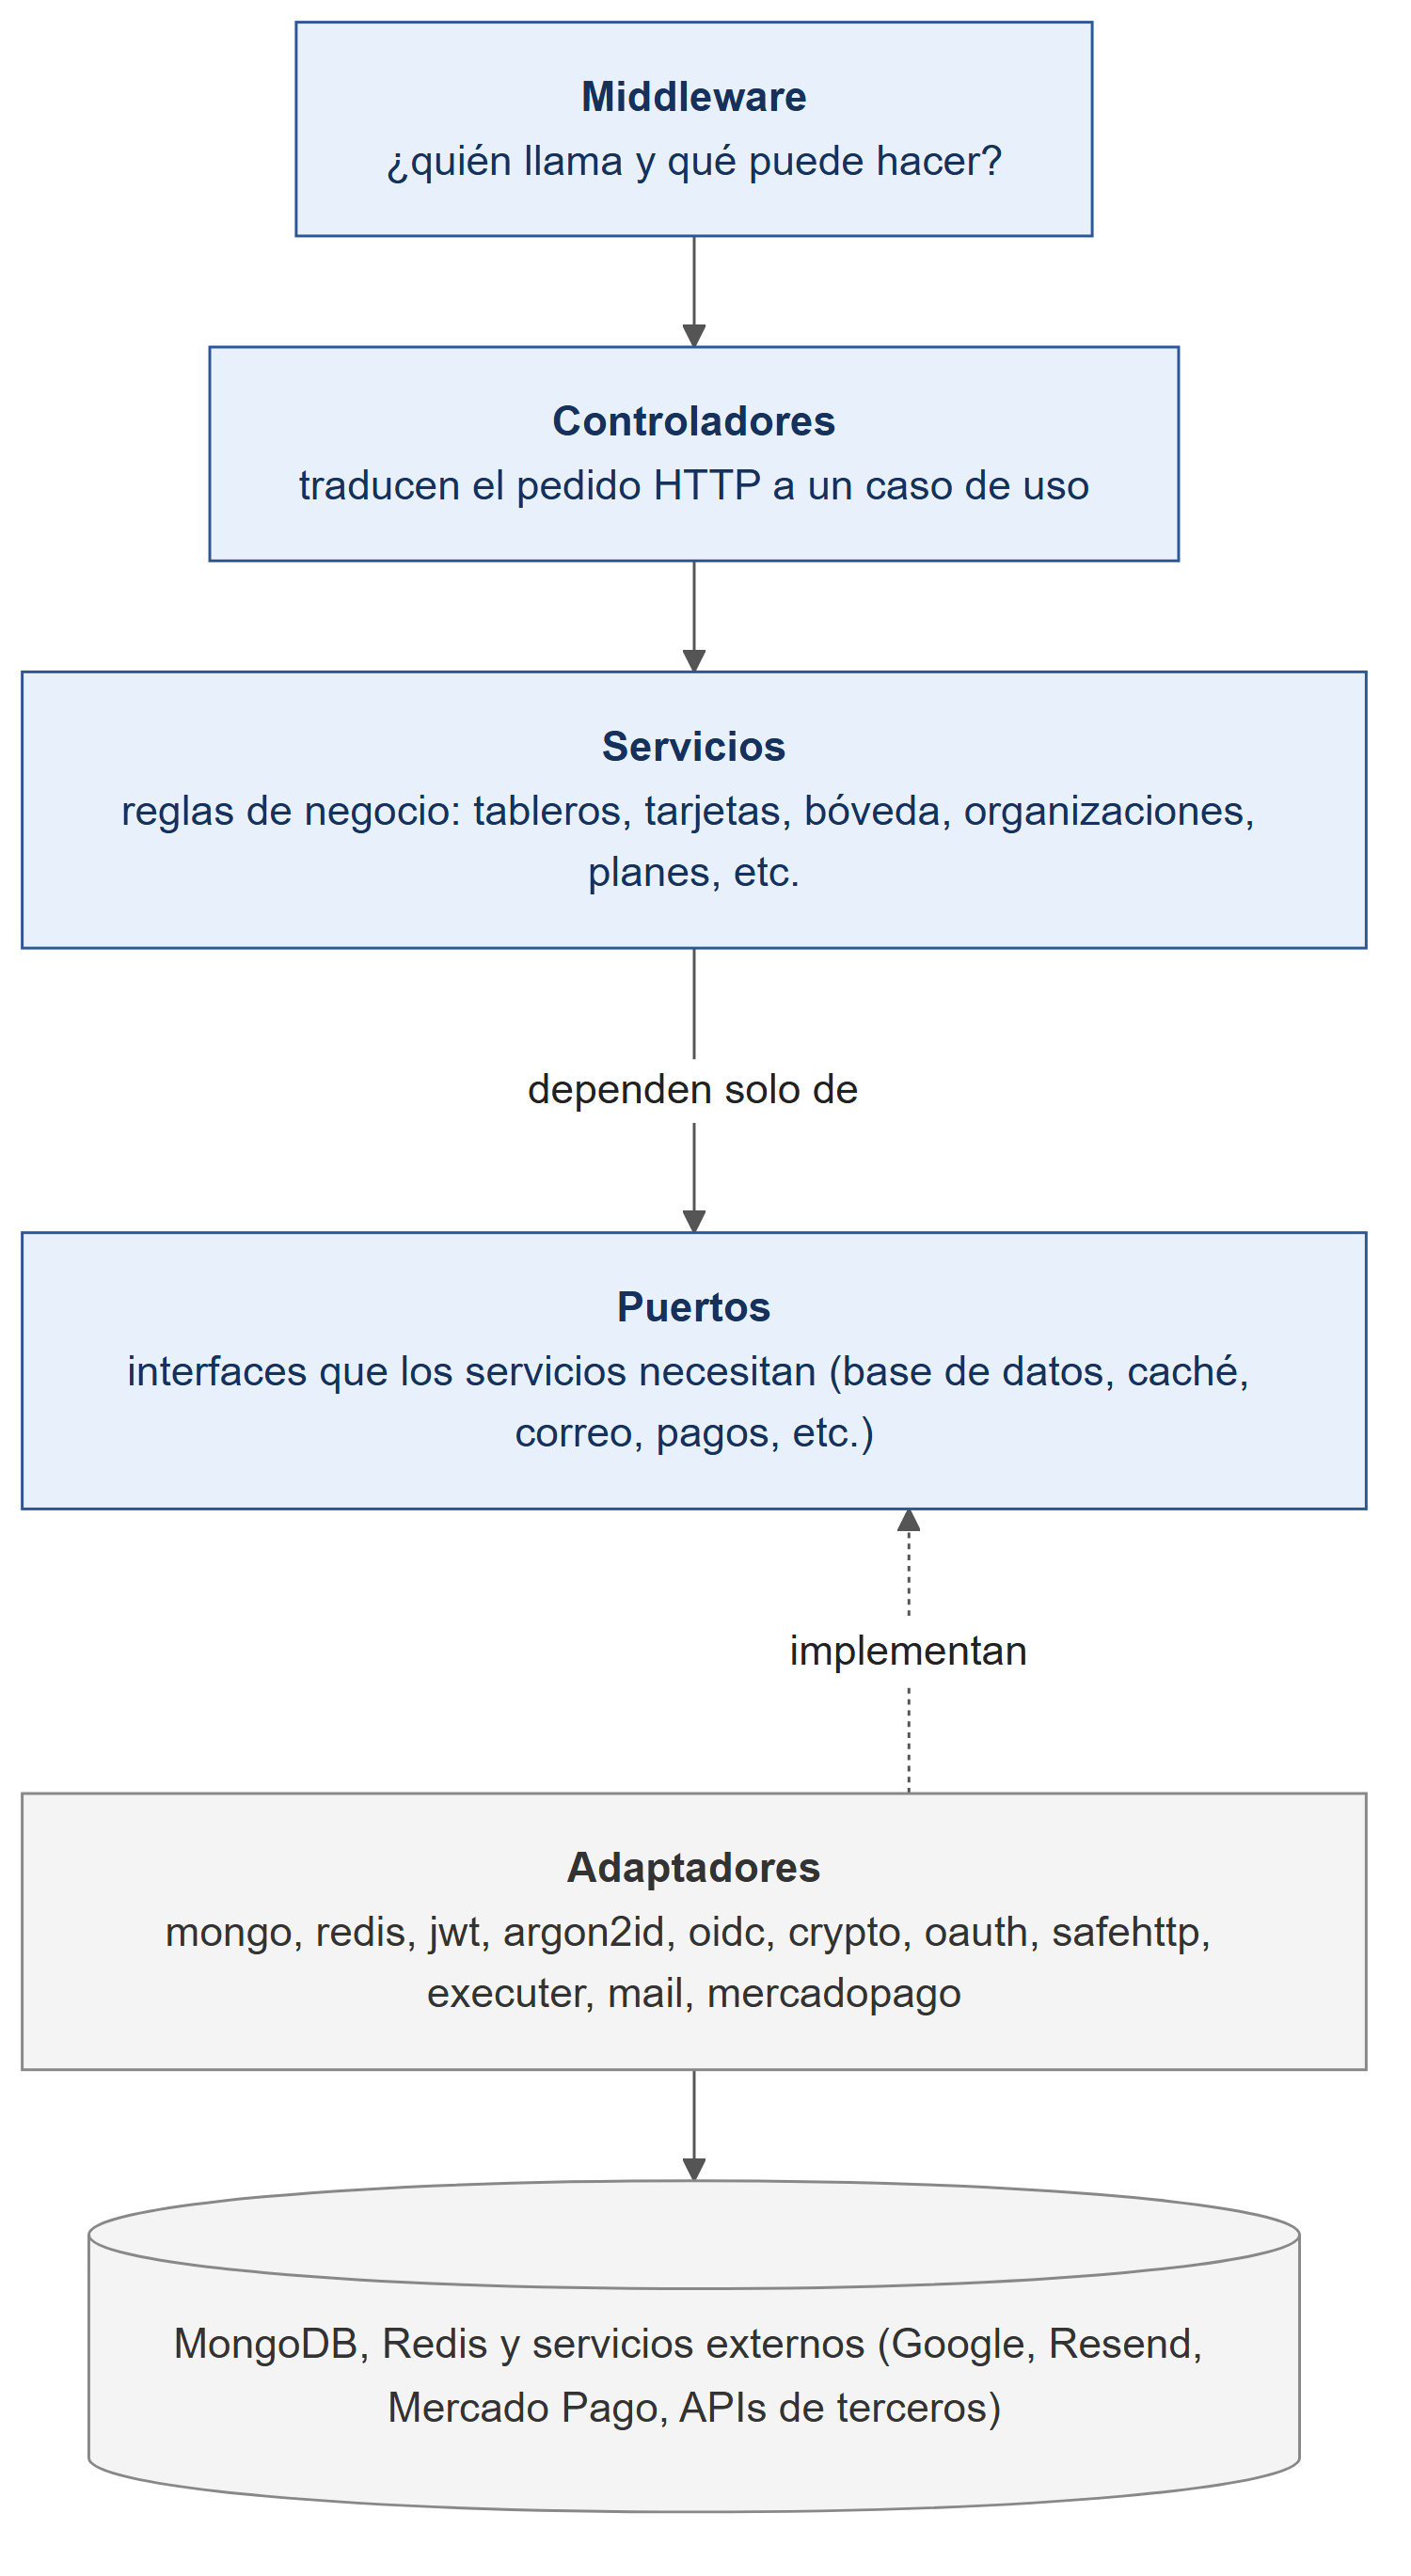
\includegraphics[width=0.65\textwidth]{figuras/fig18.png}
  \caption{Diagrama de capas del backend}
  \label{fig:capas_backend}
\end{figure}

A continuación se describen los componentes que ya se encuentran implementados en el incremento actual, indicando para cada uno su responsabilidad, su estructura en capas y los requisitos funcionales que cubre.

\section{Autenticación y Usuarios}
Este componente, materializado en los paquetes \texttt{auth} y \texttt{users}, es responsable del registro, el inicio de sesión local y federado, y la gestión del perfil propio, cubriendo los requisitos RF-01, RF-02 y RNF-02. Al igual que el resto de los componentes, se divide en controlador, servicio y adaptadores: argon2id para el hash de contraseñas, un keyring EdDSA para firmar los tokens, un cliente OIDC para Google y Redis para las sesiones y los límites de tasa.

La Figura~\ref{fig:clases_auth} presenta el diagrama de clases del componente. Los tres servicios dependen únicamente de interfaces: el almacenamiento de usuarios y sesiones, el hash de contraseñas, la firma de tokens, los límites de tasa, el envío de correos y el proveedor de identidad de Google, cuyas implementaciones concretas se encuentran en el paquete \texttt{ports}.

\begin{figure}[H]
  \centering
  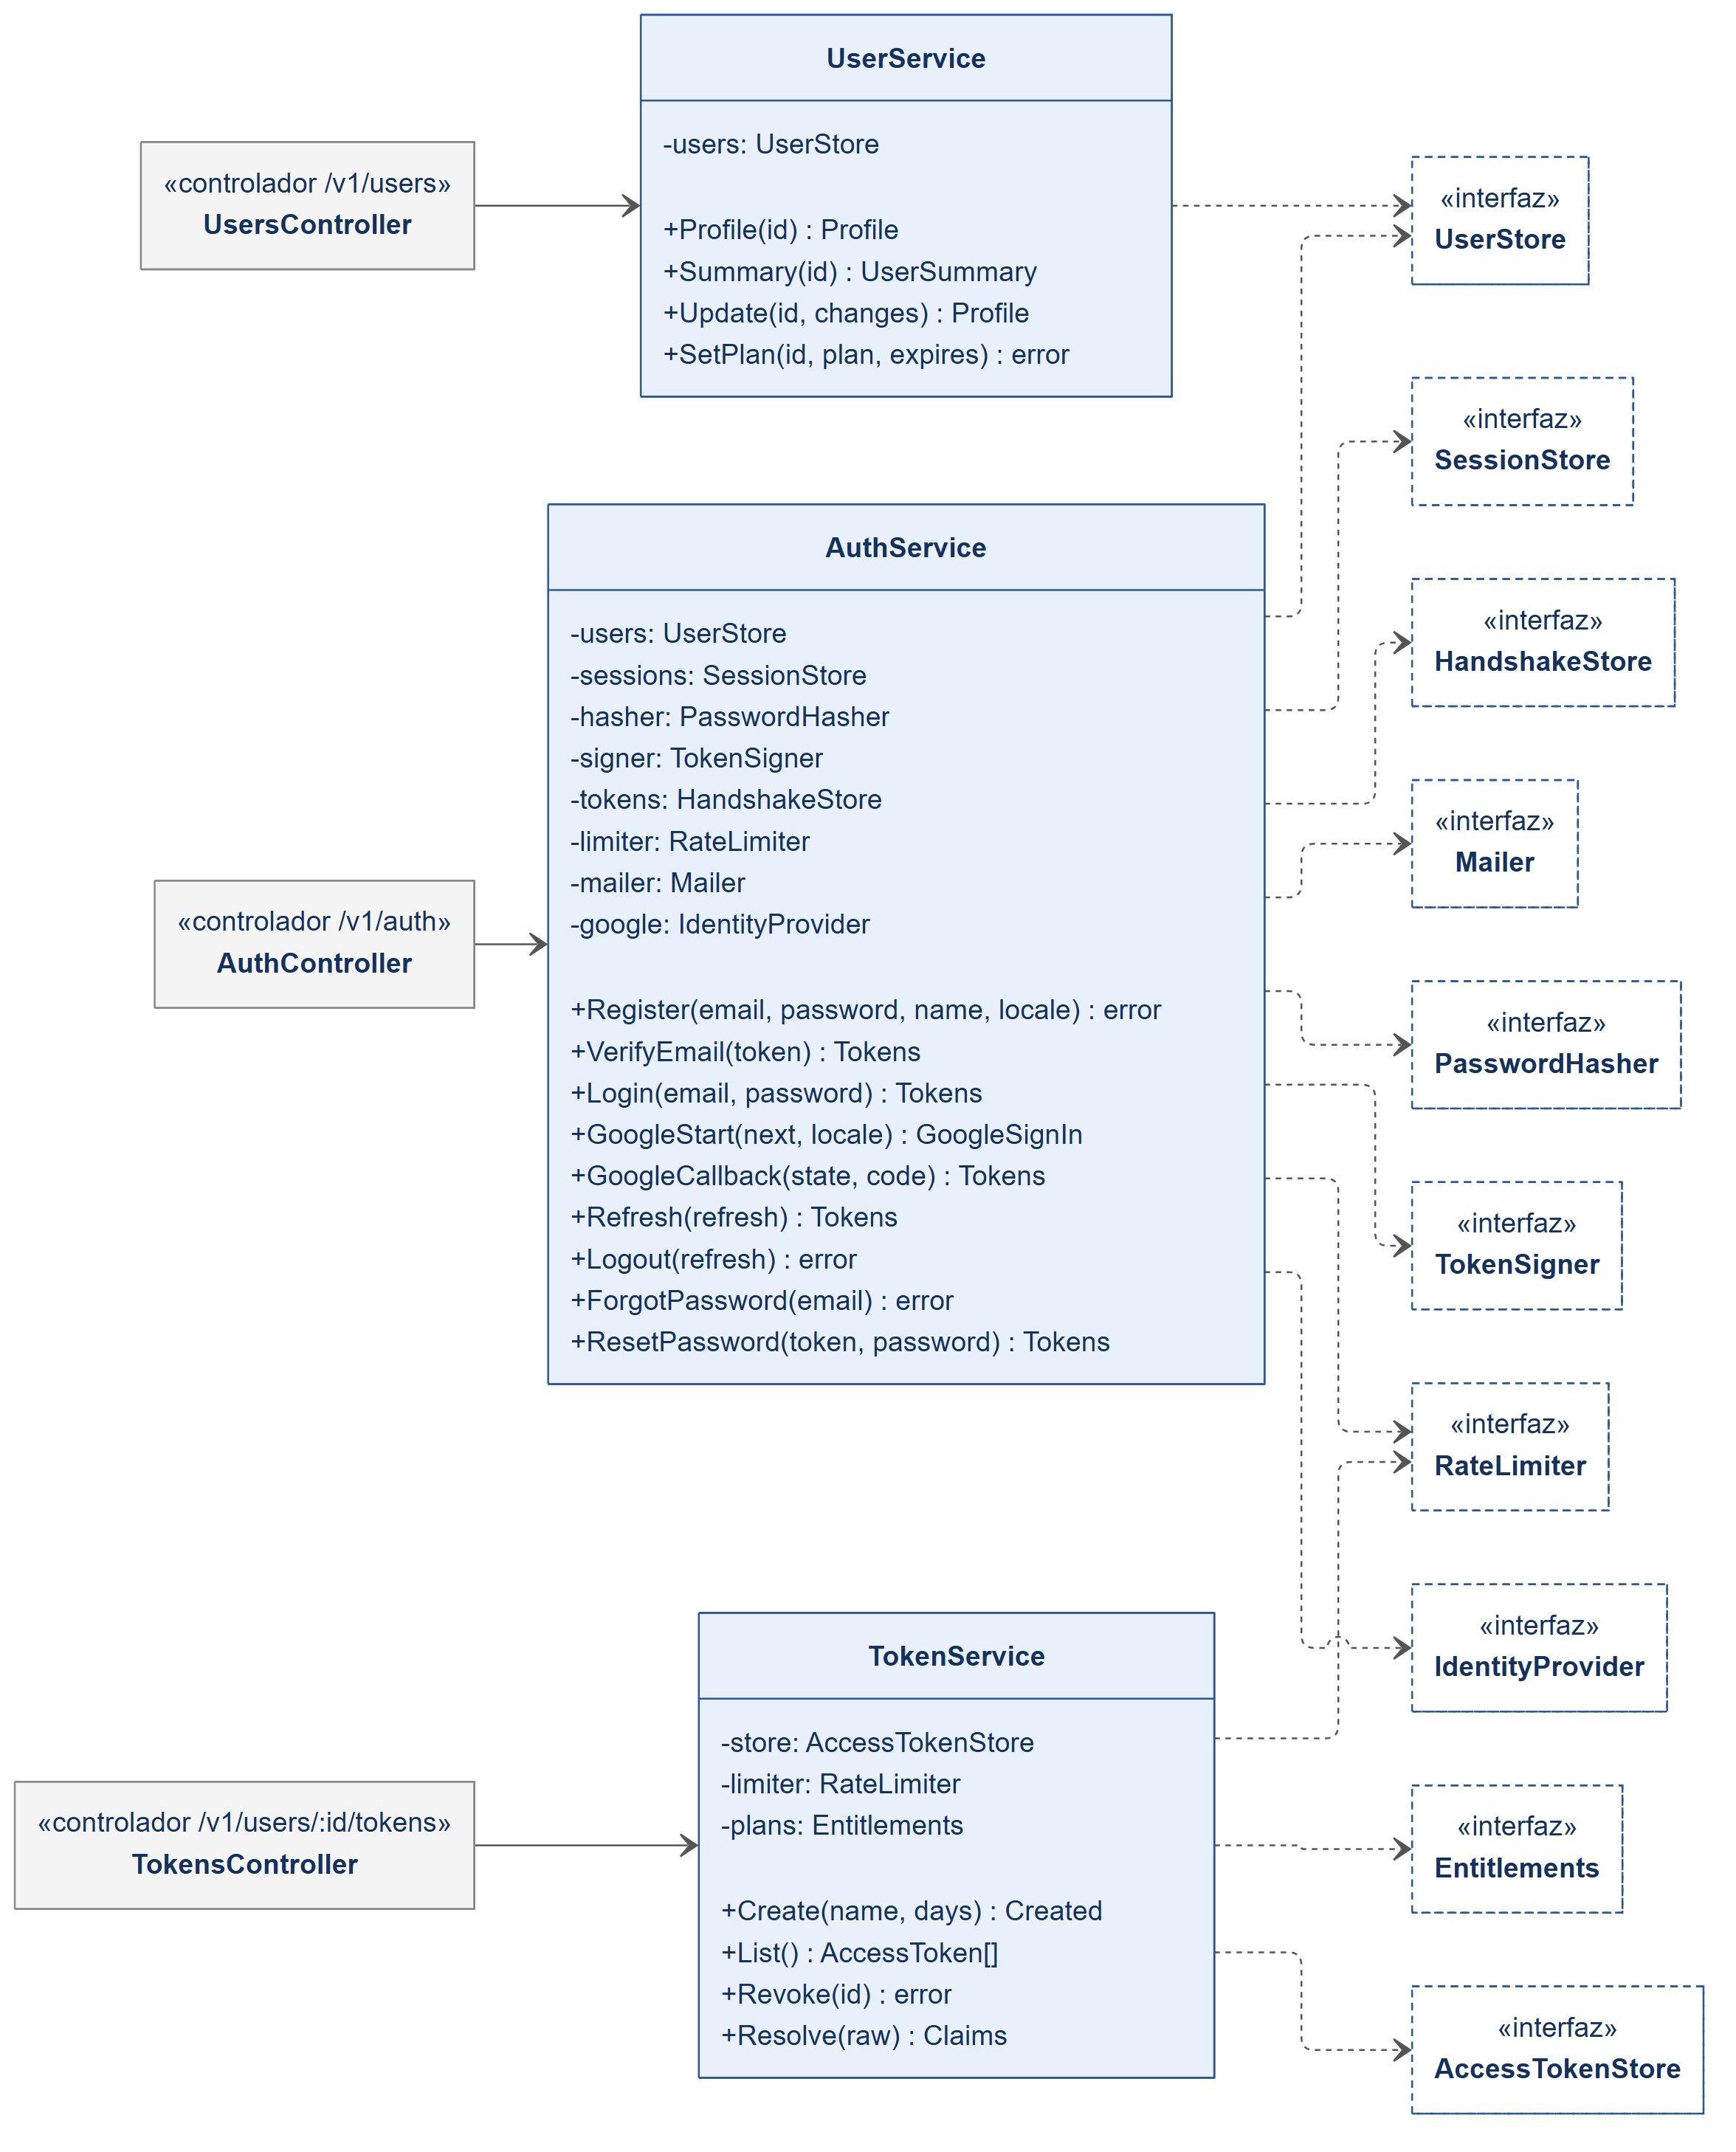
\includegraphics[width=0.92\textwidth]{figuras/fig19.png}
  \caption{Diagrama de clases de autenticación y usuarios}
  \label{fig:clases_auth}
\end{figure}

Una sesión se compone de un token de acceso JWT de quince minutos, que el frontend conserva únicamente en memoria y envía como \texttt{Authorization: Bearer}, y de un refresh token rotativo almacenado en Redis y transportado en la cookie httpOnly \texttt{tiu\_refresh}. Cada renovación emite un nuevo refresh token; si uno ya utilizado vuelve a presentarse pasado un margen de diez segundos, se revoca la familia completa de sesiones, lo que mitiga el robo de tokens. Las rutas que leen la cookie rechazan además las peticiones cross-site mediante el header \texttt{Sec-Fetch-Site}.

En la siguiente tabla se resumen los endpoints implementados para el servicio.

\begin{tablaendpoints}{Endpoints de Auth y Users}{tab:endpoints_auth}
  POST & /auth/register & Registrar una cuenta y enviar el correo de verificación. \\
  POST & /auth/verify-email & Verificar el correo con el token recibido. \\
  POST & /auth/login & Iniciar sesión con correo y contraseña. \\
  POST & /auth/refresh & Renovar la sesión a partir de la cookie de refresco. \\
  POST & /auth/logout & Cerrar la sesión y revocar el refresh token. \\
  POST & /auth/password/forgot & Solicitar el correo de recuperación de contraseña. \\
  POST & /auth/password/reset & Restablecer la contraseña con el token recibido. \\
  GET & /auth/google/start & Iniciar el flujo de inicio de sesión con Google. \\
  POST & /auth/google/callback & Completar el inicio de sesión con Google. \\
  GET & /users/\{id\} & Obtener el perfil propio, con su plan y sus límites. \\
  PATCH & /users/\{id\} & Editar el perfil propio (nombre, idioma). \\
  GET & /users/\{id\}/tokens & Listar los tokens personales propios (sin su valor). \\
  POST & /users/\{id\}/tokens & Crear un token personal (7, 15 o 30 días); su valor se muestra una única vez. \\
  DELETE & /users/\{id\}/tokens/\{token\} & Revocar un token personal. \\
  PUT & /system/users/\{id\}/plan & Asignar un plan sin pago (solo administradores). \\
\end{tablaendpoints}

Los endpoints de login, registro y recuperación aplican límites de tasa tanto por dirección de origen como por cuenta, respondiendo 429 al superarlos, lo que dificulta los ataques de fuerza bruta y el envío masivo de correos.

Los tokens personales, en el paquete \texttt{tokens}, permiten que herramientas externas como el servidor MCP actúen en nombre de un usuario. El verificador de tokens envuelve al de los JWT, de modo que el middleware de autenticación acepta ambos: un token personal se reconoce por su prefijo \texttt{tiu\_pat\_}, se busca por su hash SHA-256 y produce un principal marcado como token, que nunca es administrador. Un segundo middleware limita ese principal a una lista explícita de rutas (lectura de tableros, tarjetas, organizaciones, el perfil y el catálogo, y creación, edición y eliminación de tableros, tarjetas e hilos), por lo que toda ruta nueva queda cerrada a los tokens hasta que se la habilite. Cada usuario puede tener hasta diez tokens activos, la creación está limitada a diez por hora, y tanto la creación como cada uso verifican que el plan del usuario incluya acceso por API.

\section{Control de acceso y organizaciones}
El control de acceso se concentra en el paquete \texttt{access}, que constituye el único lugar del sistema donde se decide el rol de un principal sobre un recurso. Los servicios nunca comparan identificadores por su cuenta, sino que consultan al puerto \texttt{infrastructure.Access} y comparan el rol obtenido con el mínimo requerido mediante \texttt{AtLeast}.

Sobre un tablero existen tres roles jerárquicos: \texttt{owner}, \texttt{editor} y \texttt{viewer}. Los viewers pueden leer el tablero, sus miembros y los resultados de las tarjetas; los editors pueden además crear, editar, mover y eliminar tarjetas y dibujar hilos; finalmente, el owner puede también renombrar, eliminar y compartir el tablero. Por debajo del rol que una ruta requiere, el tablero responde 404.

Por su parte, las organizaciones, en el paquete \texttt{orgs}, funcionan como un tenant mínimo con roles \texttt{admin} y \texttt{member}. Un tablero creado dentro de una organización alcanza a todos sus miembros sin necesidad de compartirlo: los admins actúan como owners y los members como viewers, prevaleciendo el mayor entre ese rol y el asignado explícitamente en el tablero. La invariante de que una organización conserve al menos un administrador se garantiza en el propio filtro de MongoDB, evitando condiciones de carrera entre degradaciones concurrentes, y una organización solo puede eliminarse cuando ningún tablero ni grupo la referencia. Cada organización tiene además un pagador, su dueño o en su defecto su primer administrador, cuyo plan determina los límites de la organización y de sus tableros.

Los grupos, en el paquete \texttt{groups}, agrupan usuarios con el propósito principal de compartir secretos. En un grupo perteneciente a una organización, los admins actúan como owners y los members solo lo ven, de modo que los secretos del grupo permanecen restringidos a las personas que este lista.

Las clases que intervienen se muestran en la Figura~\ref{fig:clases_access}. El \texttt{Resolver} implementa el puerto \texttt{Access} que consultan los demás servicios para conocer el rol de un principal, mientras que \texttt{OrgService} y \texttt{GroupService} gestionan los miembros y delegan en el puerto \texttt{ScopePurger} la eliminación de los secretos de quien deja de pertenecer. Ambos servicios consultan además el puerto \texttt{Entitlements} para rechazar, con 402, la creación de organizaciones o grupos y el ingreso de miembros que excedan el plan correspondiente.

\begin{figure}[H]
  \centering
  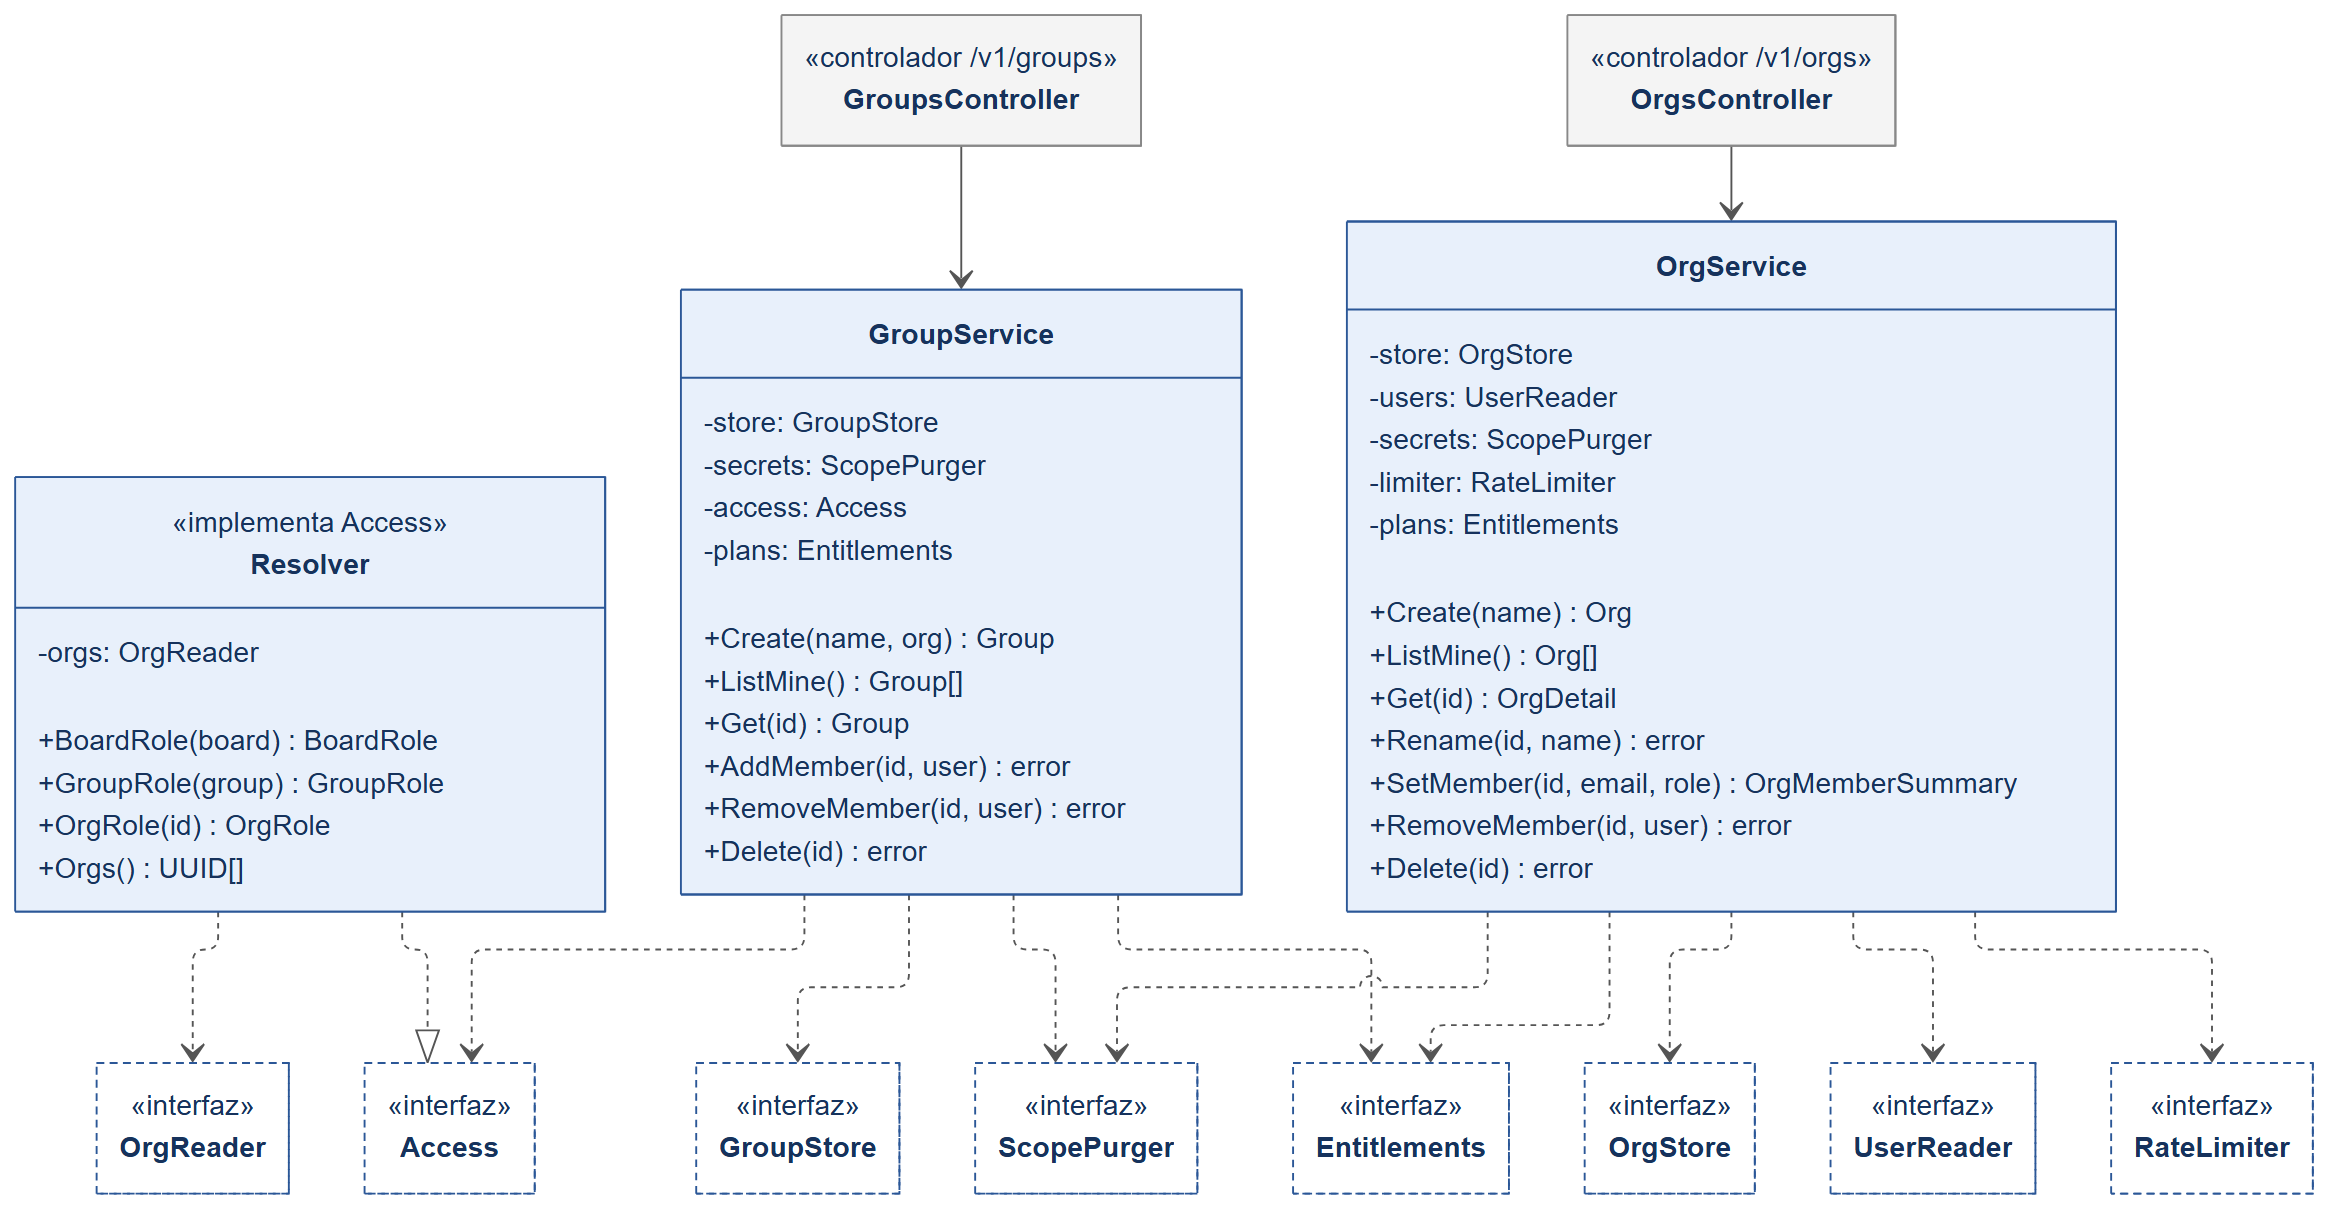
\includegraphics[width=0.95\textwidth]{figuras/fig20.png}
  \caption{Diagrama de clases de control de acceso y organizaciones}
  \label{fig:clases_access}
\end{figure}

\begin{tablaendpoints}{Endpoints de Orgs y Groups}{tab:endpoints_orgs_groups}
  GET & /orgs & Listar las organizaciones del usuario. \\
  POST & /orgs & Crear una organización. \\
  GET & /orgs/\{id\} & Obtener una organización con sus miembros, su plan y su uso. \\
  PATCH & /orgs/\{id\} & Renombrar la organización. \\
  DELETE & /orgs/\{id\} & Eliminar la organización si está vacía. \\
  PUT & /orgs/\{id\}/members & Agregar un miembro por correo o cambiar su rol. \\
  DELETE & /orgs/\{id\}/members/\{user\} & Quitar un miembro o abandonar la organización. \\
  GET & /groups & Listar los grupos del usuario. \\
  POST & /groups & Crear un grupo (opcionalmente dentro de una organización). \\
  GET & /groups/\{id\} & Obtener un grupo. \\
  DELETE & /groups/\{id\} & Eliminar el grupo y purgar sus secretos. \\
  POST/DELETE & /groups/\{id\}/members & Agregar/quitar un miembro. \\
\end{tablaendpoints}

\section{Gestión de Tableros}
Este componente, materializado en el paquete \texttt{boards}, es responsable del CRUD de tableros, de la gestión de miembros por rol y de las conexiones (\texttt{strands}) entre tarjetas, cubriendo los requisitos RF-04 y RF-06. Internamente se divide en tres capas bien diferenciadas.

El controlador, en \texttt{controllers/boards/controllers.go}, expone los endpoints REST bajo \texttt{/v1/boards}. El servicio, en \texttt{services/boards/main.go}, verifica el rol del llamante a través del puerto \texttt{Access}, orquesta las operaciones de dominio y delega la persistencia en el puerto \texttt{infrastructure.Database}, sin acoplarse a ninguna tecnología concreta. Finalmente, el adaptador en \texttt{ports/mongo/mon.go} provee la implementación concreta sobre MongoDB.

Esta estructura se refleja en la Figura~\ref{fig:clases_boards}, donde \texttt{BoardService} depende de los puertos \texttt{Database} y \texttt{Access} para persistir y autorizar, de \texttt{UserReader} para resolver a los miembros por correo, de \texttt{ScopePurger} para purgar sus secretos, de \texttt{RateLimiter} para limitar las invitaciones, de \texttt{OrgReader} para conocer la organización del tablero y de \texttt{Entitlements} para aplicar los límites del plan de quien lo paga.

\begin{figure}[H]
  \centering
  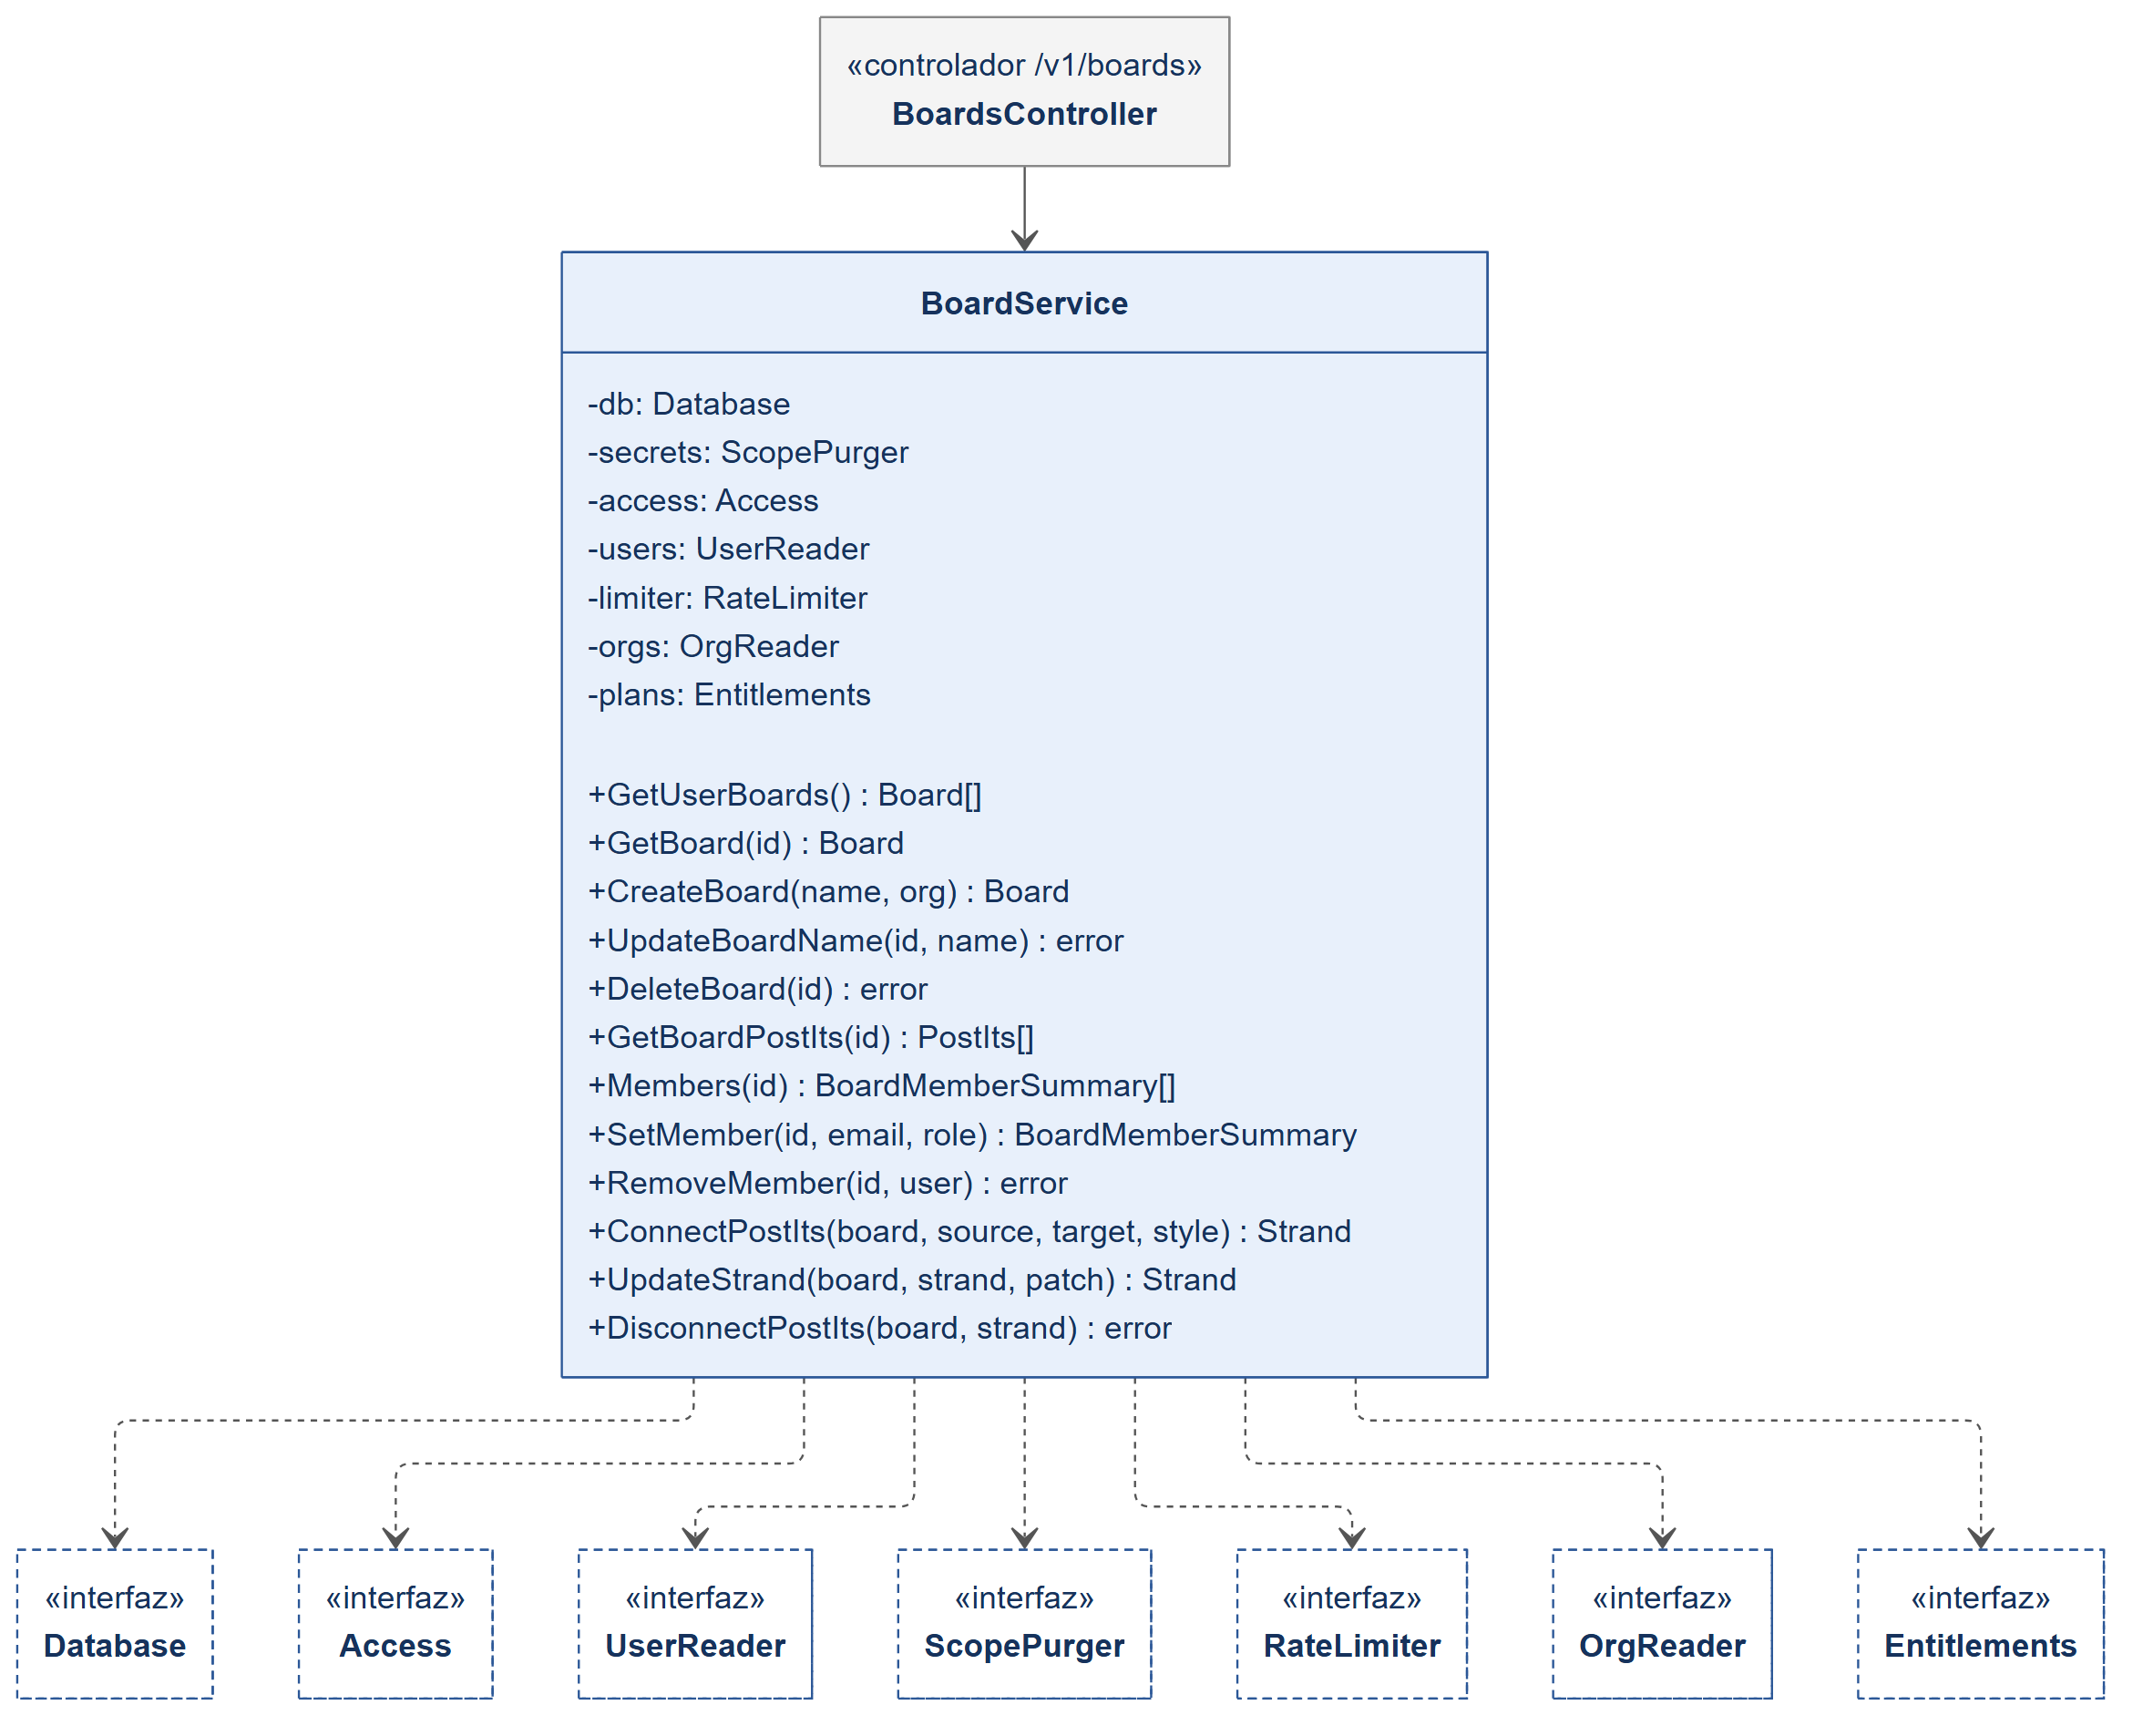
\includegraphics[width=0.82\textwidth]{figuras/fig21.png}
  \caption{Diagrama de clases de gestión de tableros}
  \label{fig:clases_boards}
\end{figure}

En la siguiente tabla se resumen los endpoints implementados para el servicio.

\begin{tablaendpointsrol}{Endpoints de Boards}{tab:endpoints_boards}
  GET & /boards & Listar los tableros propios, compartidos y de las organizaciones del usuario. & — \\
  GET & /boards/\{id\} & Obtener un tablero junto con el rol del llamante. & viewer \\
  POST & /boards & Crear tablero (name, org opcional). & — \\
  DELETE & /boards/\{id\} & Eliminar tablero, sus post-its y purgar sus secretos y claves. & owner \\
  GET & /boards/\{id\}/post-its & Listar post-its asociados. & viewer \\
  PATCH & /boards/\{id\}/name & Renombrar tablero. & owner \\
  GET & /boards/\{id\}/members & Listar los miembros con su rol. & viewer \\
  PUT & /boards/\{id\}/members & Agregar un miembro por correo o cambiar su rol. & owner \\
  DELETE & /boards/\{id\}/members/\{user\} & Quitar un miembro, o abandonar el tablero si es el propio usuario. & owner (o el propio miembro) \\
  POST & /boards/\{id\}/strands & Crear hilo entre dos tarjetas, opcionalmente con su estilo. & editor \\
  PATCH & /boards/\{id\}/strands/\{strand\} & Cambiar el estilo de un hilo (etiqueta, flechas, grosor y color). & editor \\
  DELETE & /boards/\{id\}/strands/\{strand\} & Eliminar un hilo. & editor \\
\end{tablaendpointsrol}

Para garantizar la consistencia del modelo de datos, las operaciones mutacionales sobre el tablero fueron diseñadas priorizando la integridad referencial y la atomicidad. La creación de conexiones, en \texttt{ConnectPostIts}, implementa el modificador \texttt{\$addToSet} para prevenir relaciones duplicadas e incorpora una validación estructural mediante el operador \texttt{\$all}, garantizando que tanto el nodo origen como el destino existan previamente en el documento y mitigando así la aparición de hilos colgantes.

Asimismo, la modificación del estilo de un hilo, en \texttt{UpdateStrand}, actualiza únicamente los campos enviados mediante los operadores posicionales \texttt{\$set} y \texttt{\$unset}, de modo que un valor por defecto nunca se almacena, y valida la etiqueta, las flechas, el grosor y el color antes de persistirlos.

Por su parte, la eliminación, en \texttt{DeletePostIt}, preserva la integridad del grafo delegando la limpieza de referencias al motor de la base de datos en una única operación atómica: mediante el uso de \texttt{\$pull} combinado con \texttt{\$or} se remueve simultáneamente el post-it y cualquier strand que lo involucre, asegurando la consistencia sin necesidad de orquestar múltiples transacciones. De manera análoga, \texttt{SetBoardMember} sólo agrega un miembro cuando este aún no figura en la lista, de forma que dos invitaciones concurrentes nunca lo dupliquen.

Finalmente, quitar a un miembro o eliminar el tablero desencadena la purga de los secretos que ese miembro guardaba para sí en el tablero, junto con sus claves de datos, evitando que queden credenciales huérfanas.

Las operaciones de creación consultan además el plan de quien paga el tablero, su dueño o el pagador de su organización. Crear un tablero verifica la cantidad de tableros del espacio, y agregar una persona verifica la cantidad de asientos. Al superar un límite, la operación responde 402 indicando qué límite se alcanzó, pero nunca se elimina lo que ya existe. La respuesta de un tablero informa sus límites, los asientos ocupados y los secretos disponibles, para que el frontend anticipe estas restricciones.

\section{Motor de Tarjetas}
El motor de tarjetas, en el paquete \texttt{postits}, se encarga de crear, configurar, mover y ejecutar tarjetas, cubriendo los requisitos RF-05, RF-07, RF-08, RF-12 y la configuración del rate de RF-09.

El principio de diseño central de este componente es que una tarjeta constituye una descripción declarativa de cómo obtener un dato y no un fragmento de código. El motor se limita a sustituir variables, ejecutar la petición y aplicar la proyección con jq. Esta restricción es, precisamente, lo que permite cumplir el RNF-04: agregar una integración predefinida se reduce a cargar su definición en el catálogo, sin necesidad de escribir lógica nueva ni desplegar una nueva versión del backend.

Las escrituras sobre una tarjeta actúan en nombre del llamante. Al crearla, o cada vez que cambian sus \texttt{params} o \texttt{bindings}, se registra en el campo \texttt{RunAs} la identidad de quien la configuró, y es con esa identidad que luego se resuelven sus credenciales. Esto impide que un editor utilice, a través de una tarjeta, secretos a los que no tiene acceso, y garantiza que degradar a un usuario a viewer detenga las tarjetas que se ejecutan en su nombre.

Una tarjeta personalizada, que no proviene del catálogo ni de una plantilla, define su propia petición, y el servicio la valida al crearla y al editarla: la URL debe usar \texttt{http} o \texttt{https}, el método puede ser \texttt{GET} o \texttt{POST} (este último con un cuerpo JSON de hasta 16 KB), la respuesta se interpreta como JSON o HTML, debe haber al menos una salida, y no puede haber más de veinte headers, parámetros o salidas. La petición de una tarjeta creada desde el catálogo o una plantilla, en cambio, es fija. Toda creación verifica además el límite de tarjetas por tablero del plan.

El estilo visual de cada tarjeta, correspondiente al RF-12, se guarda junto a su entrada en el documento del tablero, por lo que llega a los demás usuarios por el mismo canal de tiempo real que el resto de los cambios del tablero. La operación \texttt{StylePostIt}, reservada a los editores, valida el color, el borde, la alineación del texto y el tamaño, redondea las dimensiones a píxeles enteros dentro de los límites admitidos y actualiza únicamente los campos enviados mediante los operadores posicionales \texttt{\$set} y \texttt{\$unset}, de modo que un valor por defecto nunca se almacena.

En la Figura~\ref{fig:clases_postits} se observa que \texttt{PostItsService} no conoce el motor de integraciones concreto: depende del puerto \texttt{Executer}, implementado por el adaptador \texttt{DewIt}, del puerto \texttt{Cache} para el resultado de cada tarjeta y del puerto \texttt{SecretResolver} para obtener las credenciales en nombre de \texttt{RunAs}. Además, consulta el catálogo (\texttt{WellKnownReader}) y las plantillas (\texttt{PostitTemplates}) para crear tarjetas a partir de ellos, el puerto \texttt{Entitlements} para aplicar el límite de tarjetas por tablero y el tiempo mínimo en caché del plan, y \texttt{RateLimiter} para limitar las actualizaciones forzadas.

\begin{figure}[H]
  \centering
  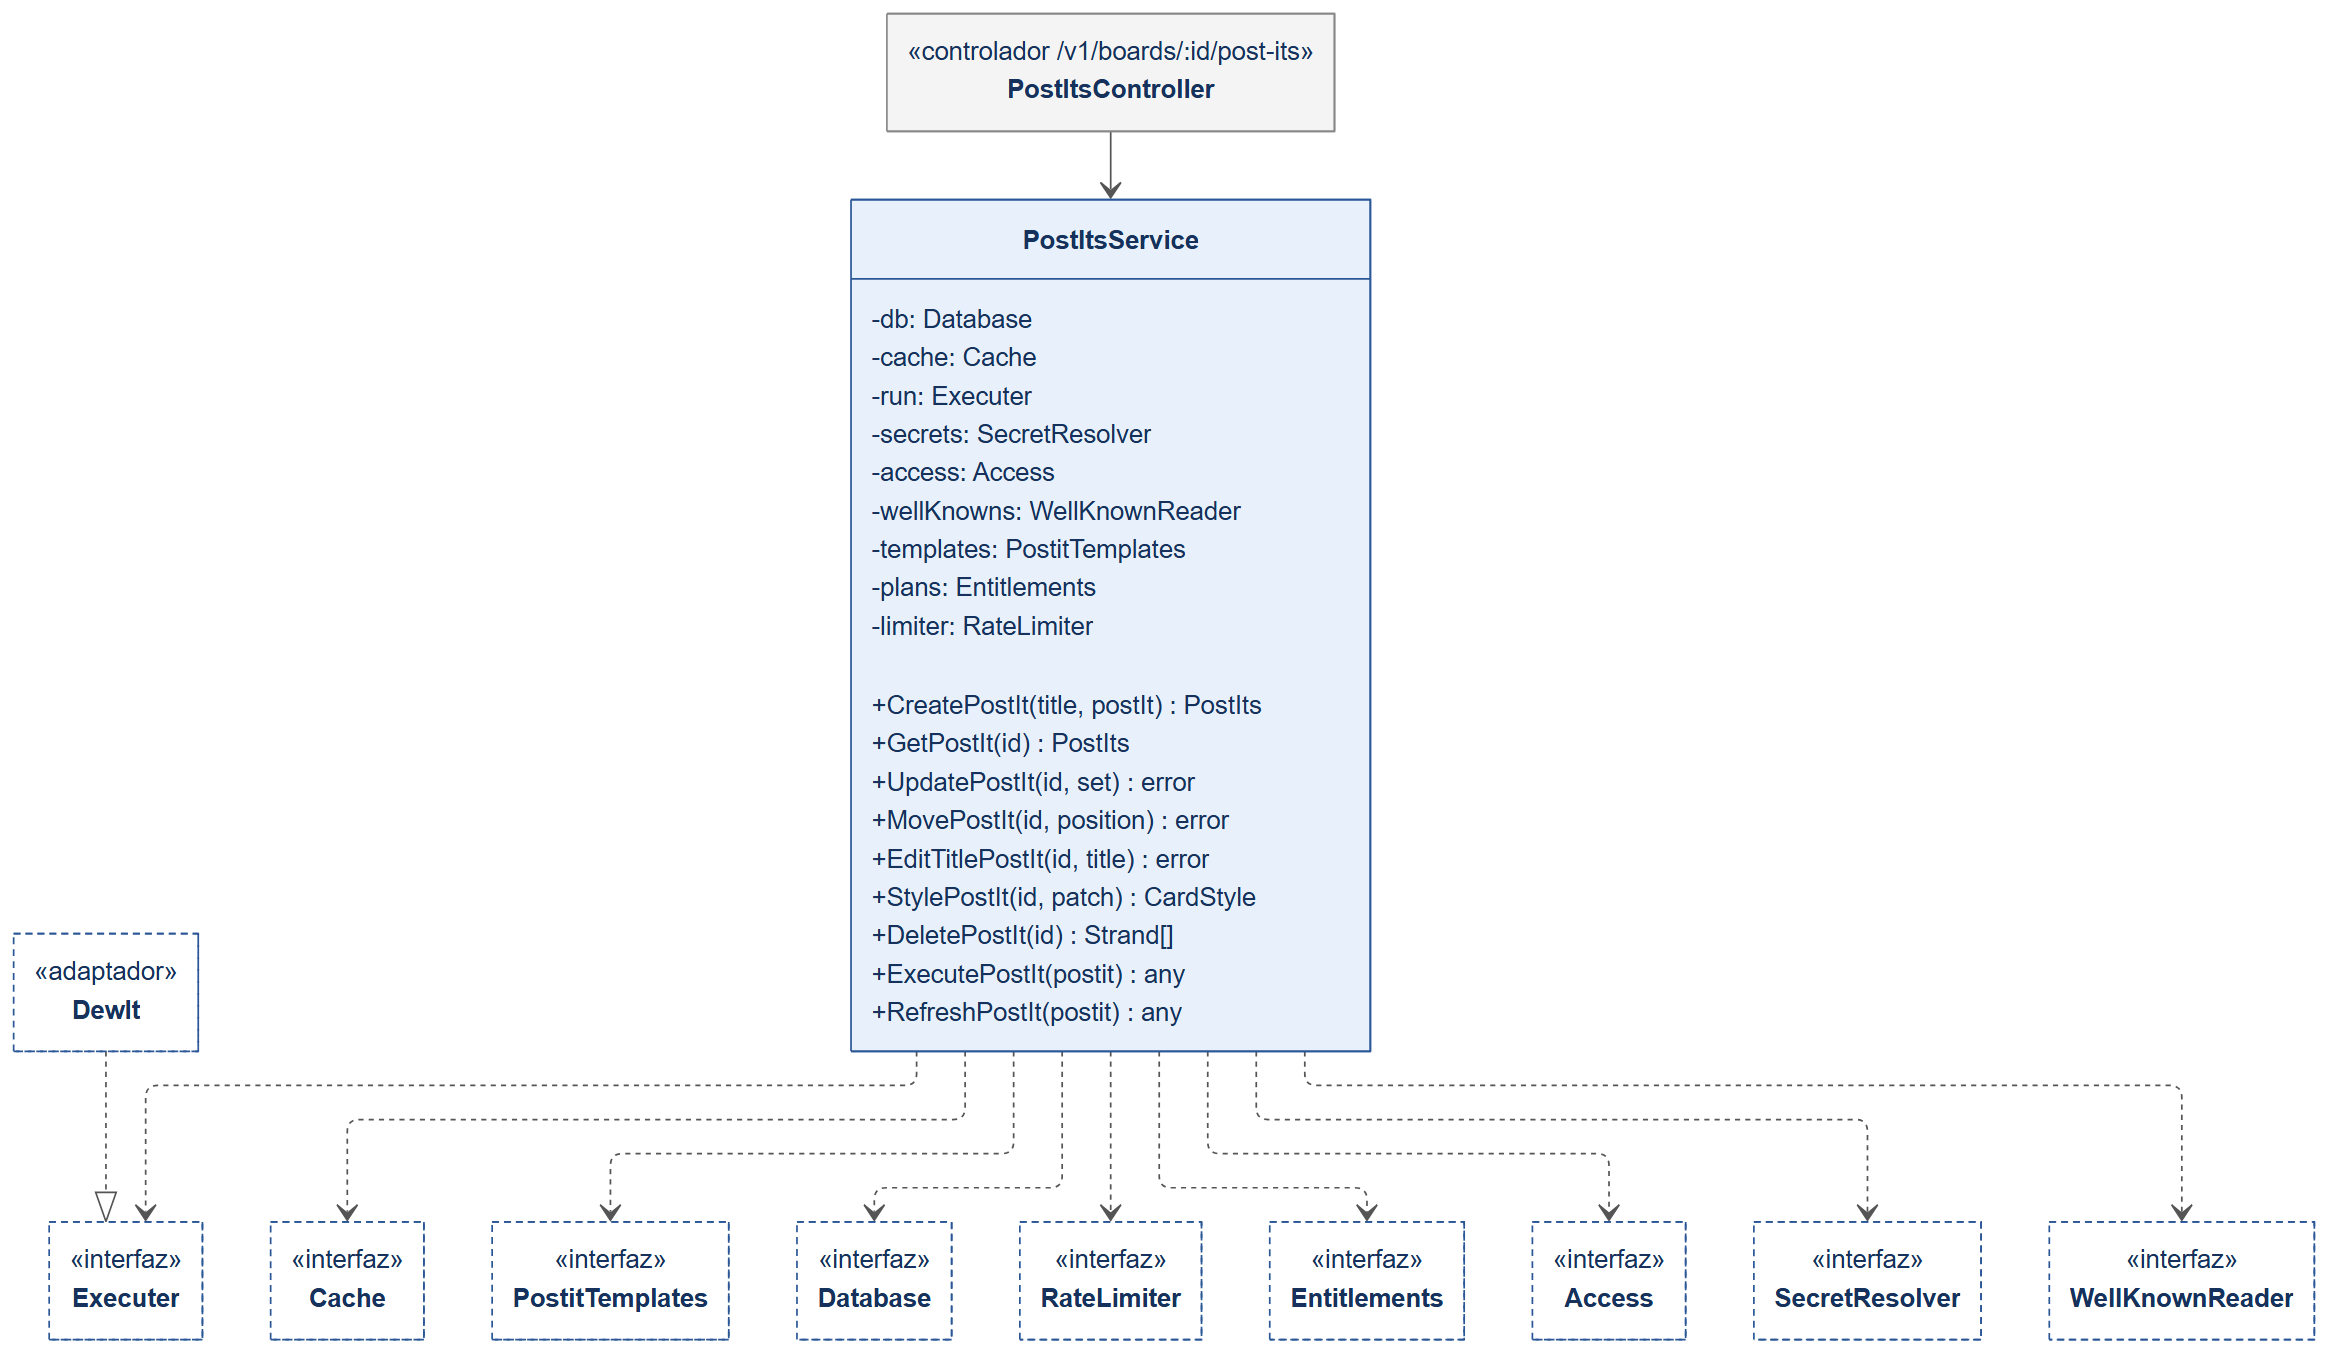
\includegraphics[width=0.95\textwidth]{figuras/fig22.png}
  \caption{Diagrama de clases del motor de tarjetas}
  \label{fig:clases_postits}
\end{figure}

Sus endpoints se resumen en la siguiente tabla.

\begin{tablaendpointsrol}{Endpoints de PostIts}{tab:endpoints_postits}
  POST & /post-its & Crear tarjeta (eventualmente desde un well-known). & editor \\
  GET & /post-its/\{id\} & Ejecutar la tarjeta y devolver el dato proyectado. & viewer \\
  GET & /post-its/\{id\}/settings & Obtener la configuración. & viewer \\
  PATCH & /post-its/\{id\}/settings & Editar params, bindings, query, response o rate, y para las tarjeta personalizada, también la URL y la petición. & editor \\
  PATCH & /post-its/\{id\}/position & Mover la tarjeta dentro del board. & editor \\
  PATCH & /post-its/\{id\}/title & Editar el título de la tarjeta. & editor \\
  PATCH & /post-its/\{id\}/style & Cambiar el estilo visual de la tarjeta (color, borde, alineación del texto y tamaño). & editor \\
  DELETE & /post-its/\{id\} & Eliminar la tarjeta y desreferenciar del board. & editor \\
\end{tablaendpointsrol}

\section{Integración con APIs}
El motor de integración, en el paquete \texttt{executer}, es responsable de resolver un PostIt a un valor concreto, cubriendo la capa de ejecución de los requisitos RF-07 y RF-08. Antes de invocarlo, el servicio de tarjetas prepara una copia del PostIt: cada placeholder \texttt{\$TOKEN} presente en \texttt{params}, \texttt{headers}, \texttt{queries} o en un valor del cuerpo JSON se mapea a una referencia de secreto, tomando el binding explícito de la tarjeta si existe. Esas referencias se resuelven como el principal \texttt{RunAs}, verificando nuevamente que pueda utilizarlas, y por último se inyectan los secretos de sistema que requiera el well-known. A continuación, cada llamada a \texttt{DewIt.Execute} recorre seis pasos.

En primer lugar, un short-circuit estático: si el campo \texttt{Resource} es nil, se devuelven los \texttt{Params} tal cual, lo que da soporte a las integraciones \texttt{static\_card} e \texttt{image} y a cualquier tarjeta sin fuente externa. Luego se elige el intérprete según el campo \texttt{response}: JSON con \texttt{gojq} o HTML con \texttt{goquery}. A continuación, la sustitución de variables, en la que \texttt{populate} reemplaza dentro de las queries y los headers aquellos valores cuyo contenido coincida con el nombre de un Param, identificados por el prefijo \texttt{\$}. En una petición \texttt{POST}, el cuarto paso aplica la misma sustitución a cada valor de texto del cuerpo JSON.

El quinto paso es la petición HTTP, creada con un \texttt{context.WithTimeout} de diez segundos, ensamblando querystring, headers y, si corresponde, el cuerpo como \texttt{application/json}, y exigiendo un status 200 OK; cualquier otro código se reporta como error de la tarjeta. Por último, el cuerpo de la respuesta, leído hasta un máximo de 2MB, se interpreta con el parser elegido: para JSON se compila cada expresión con \texttt{gojq.Parse} y se ejecuta con un timeout de doscientos cincuenta milisegundos, mientras que para HTML cada valor es un selector jquery evaluado con \texttt{goquery}, devolviendo al servicio un objeto con un valor por clave.

La siguiente tabla detalla las integraciones predefinidas que el sistema carga inicialmente en el catálogo.

\begingroup
\footnotesize
\setlength{\tabcolsep}{4.5pt}
\renewcommand{\arraystretch}{1.35}
\rowcolors{2}{gray!7}{white}
\begin{longtable}{
  >{\ttfamily\raggedright\arraybackslash}p{\dimexpr 0.21\textwidth - 2\tabcolsep\relax}
  >{\raggedright\arraybackslash}p{\dimexpr 0.20\textwidth - 2\tabcolsep\relax}
  >{\raggedright\arraybackslash}p{\dimexpr 0.33\textwidth - 2\tabcolsep\relax}
  >{\centering\arraybackslash}p{\dimexpr 0.10\textwidth - 2\tabcolsep\relax}
  >{\raggedright\arraybackslash}p{\dimexpr 0.16\textwidth - 2\tabcolsep\relax}
}
  \toprule
  \rowcolor{gray!18}
  \normalfont\bfseries Clave & \bfseries Fuente & \bfseries Query & \bfseries Rate & \bfseries Credencial \\
  \midrule
  \endfirsthead
  \toprule
  \rowcolor{gray!18}
  \normalfont\bfseries Clave & \bfseries Fuente & \bfseries Query & \bfseries Rate & \bfseries Credencial \\
  \midrule
  \endhead
  \midrule
  \rowcolor{white}
  \multicolumn{5}{r}{\textit{\scriptsize Continúa en la página siguiente...}} \\
  \endfoot
  \bottomrule
  \caption{Integraciones predefinidas actuales}
  \label{tab:integraciones_predefinidas}
  \endlastfoot
  static\_card & Interna & — & — & — \\
  image & Interna & — & — & — \\
  temperature & Open-Meteo & mín./máx. de temperatura horaria & 30 s & — \\
  air\_quality & Open-Meteo & Índice de calidad del aire, Material particulado 2.5 y fecha y hora de medida & 15 min & — \\
  events\_search & Ticketmaster & nombre, inicio de venta, imagen, fecha, lugar, ciudad y URL del primer evento & 120 s & del usuario \\
  dog\_facts & Dog API & atributos del primer fact & 5 s & — \\
  dolar\_oficial & dolarapi.com & compra/venta & 120 s & — \\
  exchange\_rate & currencyapi.com & código, valor y fecha & 60 min & del usuario \\
  riesgo\_pais & argentinadatos.com & valor y fecha & 60 min & — \\
  crypto\_price & CoinGecko & moneda, precio y variación en 24 h & 60 s & — \\
  nasa\_apod & NASA APOD & título, imagen, explicación y fecha & 60 min & de sistema \\
  gmail\_inbox & Gmail API & mensajes no leídos y totales & 60 s & OAuth2 (Google) \\
  google\_calendar & Google Calendar API & resumen e inicio del próximo evento & 5 min & OAuth2 (Google) \\
  github\_repo & GitHub API & nombre, estrellas, forks, issues y descripción del repositorio más popular & 5 min & — \\
\end{longtable}
\endgroup

El catálogo se almacena en la colección \texttt{well\_knowns} y lo administra el servicio \texttt{wellknowns}. Cada definición contiene la petición a realizar, la query de proyección, el rate por defecto, los parámetros que debe completar el usuario y las salidas que produce, con sus textos en español e inglés, además de los secretos de sistema que necesita. Los administradores de la plataforma pueden crear, modificar, eliminar y restaurar definiciones sin desplegar una nueva versión del backend.

El rate indicado es el valor por defecto de cada definición, y el tiempo que un resultado permanece en caché nunca es menor al mínimo del plan de quien paga el tablero (600, 150 o 60 segundos en los planes Free, Pro y Max, respectivamente).

La eliminación es lógica, de modo que las tarjetas creadas a partir de una definición borrada siguen funcionando. Durante las migraciones, el sistema carga las integraciones incorporadas que todavía no figuran en la colección, sin sobrescribir las que ya existen. Los placeholders de las definiciones se escriben en minúsculas (\texttt{\$credential}, \texttt{\$api\_key}), mientras que los nombres de los secretos del usuario van en mayúsculas (\texttt{\$MY\_KEY}), lo que evita colisiones entre ambos.

Los secretos del sistema, como la clave de la API de NASA, se resuelven al momento de la ejecución y nunca se almacenan en la tarjeta. Una integración personalizada, correspondiente al RF-08, reutiliza exactamente la misma estructura \texttt{PostIts} que un well-known, con el campo \texttt{WellKnown} vacío y todos los demás campos suministrados por el usuario, lo que la vuelve fácilmente extensible.

Las plantillas de tarjeta, en el paquete \texttt{postittemplates}, permiten guardar la configuración de una integración personalizada como un tipo de tarjeta reutilizable. Cada plantilla pertenece a un usuario, a un tablero o a una organización, y su clave comienza con el prefijo \texttt{custom\_} para no confundirse con las definiciones del catálogo. Quién puede verla, usarla o modificarla depende de ese ámbito, que se resuelve a través del puerto \texttt{Access}. Al crear una tarjeta a partir de una plantilla, esta se convierte a la misma forma que una definición del catálogo, por lo que el motor la ejecuta sin distinción. A diferencia del catálogo, una plantilla está en un único idioma, siempre realiza una petición \texttt{GET} y no puede utilizar secretos del sistema. La cantidad de plantillas de cada ámbito está limitada por el plan de quien lo paga, y eliminar una plantilla es definitivo: las tarjetas creadas a partir de ella siguen funcionando con su copia, pero ya no pueden editarse.

La Figura~\ref{fig:clases_wellknowns} muestra las clases de ambos servicios. \texttt{WellKnownService} administra el catálogo, mientras que \texttt{PostitTemplateService} implementa el puerto \texttt{PostitTemplates}, que el servicio de tarjetas consulta para obtener la definición de una plantilla utilizable en un tablero.

\begin{figure}[H]
  \centering
  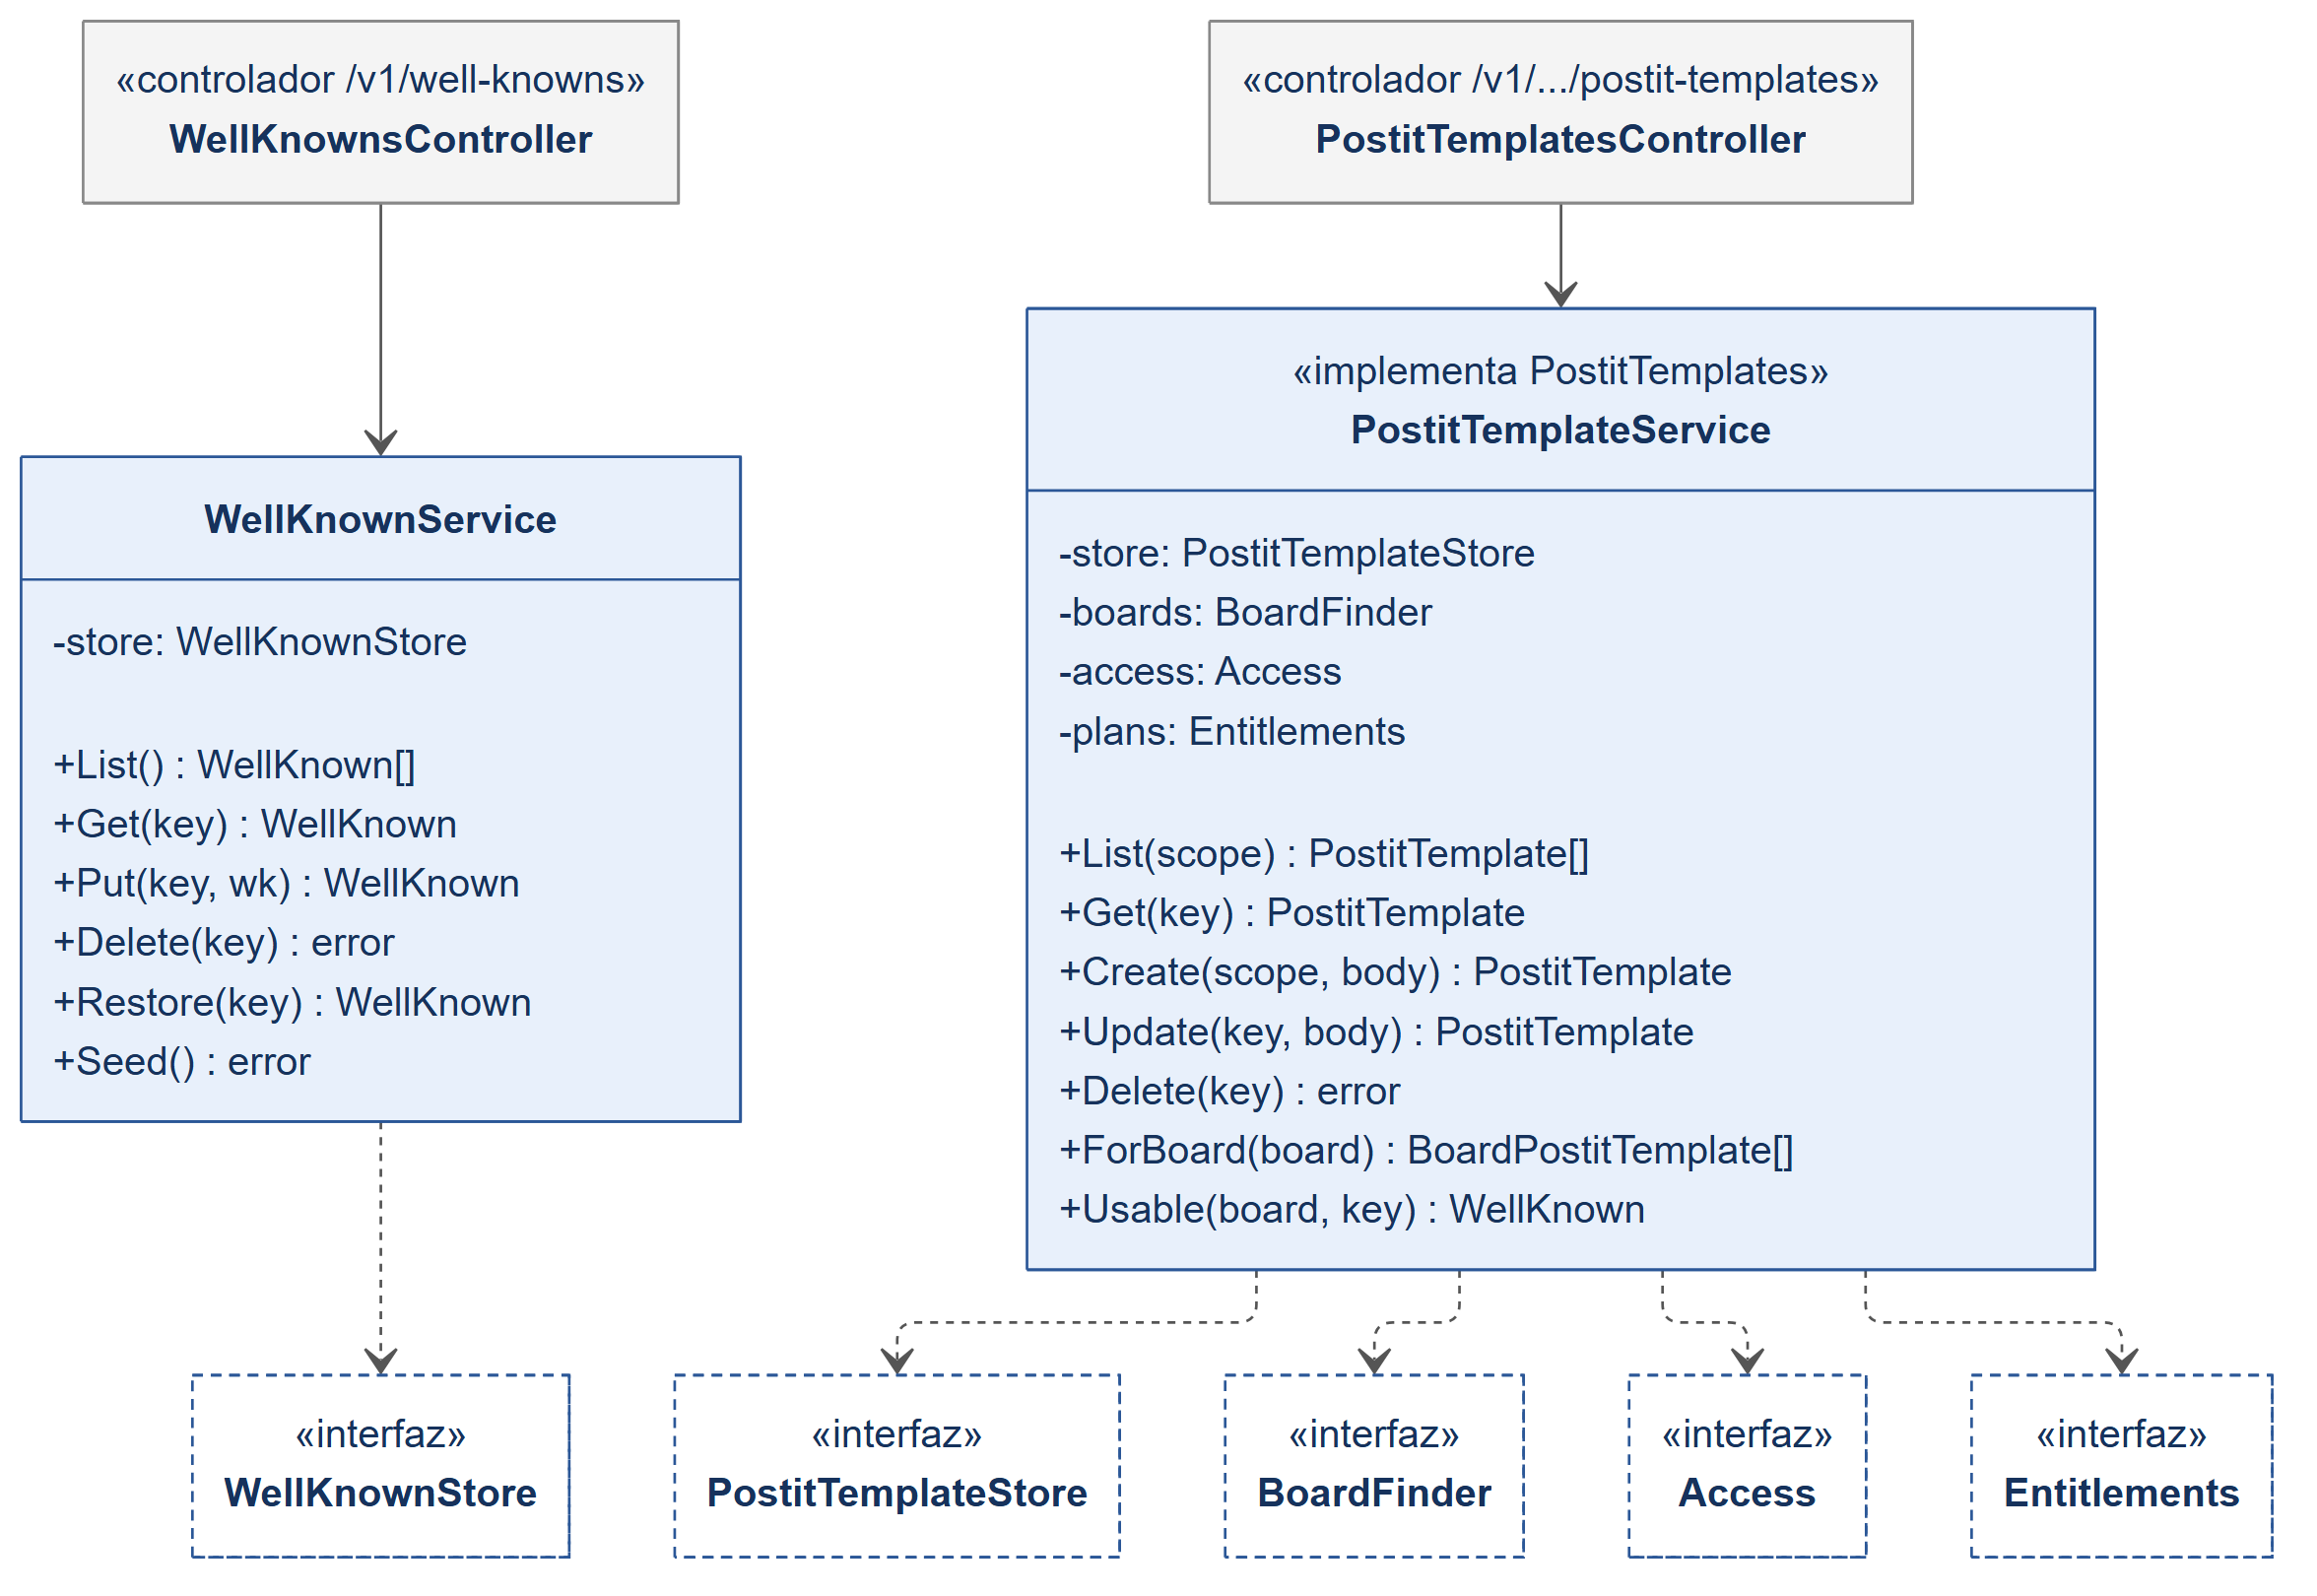
\includegraphics[width=0.92\textwidth]{figuras/fig23.png}
  \caption{Diagrama de clases del catálogo de integraciones y las plantillas de tarjeta}
  \label{fig:clases_wellknowns}
\end{figure}

Los endpoints del catálogo y de las plantillas se resumen en la Tabla~\ref{tab:endpoints_wellknowns}.

\begin{tablaendpointsrol}{Endpoints del catálogo y de las plantillas. \texttt{\{scope\}} corresponde a \texttt{/users/\{id\}}, \texttt{/boards/\{id\}} u \texttt{/orgs/\{id\}}.}{tab:endpoints_wellknowns}
  GET & /well-knowns & Listar el catálogo de integraciones. & usuario autenticado \\
  GET & /well-knowns/\{key\} & Obtener una definición del catálogo. & usuario autenticado \\
  PUT & /well-knowns/\{key\} & Crear o reemplazar una definición. & administrador \\
  DELETE & /well-knowns/\{key\} & Eliminar una definición (eliminación lógica). & administrador \\
  POST & /well-knowns/\{key\}/restore & Restaurar una definición eliminada. & administrador \\
  GET & \{scope\}/postit-templates & Listar las plantillas de un scope. & según el scope \\
  POST & \{scope\}/postit-templates & Crear una plantilla en el scope. & según el scope \\
  GET & /boards/\{id\}/postit-templates/usable & Listar las plantillas disponibles en un tablero. & viewer \\
  GET & /postit-templates/\{key\} & Obtener una plantilla. & según el scope \\
  PUT & /postit-templates/\{key\} & Modificar una plantilla. & según el scope \\
  DELETE & /postit-templates/\{key\} & Eliminar una plantilla. & según el scope \\
\end{tablaendpointsrol}

\section{Bóveda de secretos}
La bóveda, en el paquete \texttt{secrets}, es responsable de almacenar las credenciales que las tarjetas necesitan para consultar APIs privadas y de decidir quién puede gestionarlas, verlas y utilizarlas. Un secreto se identifica por su ámbito y su nombre, donde el ámbito puede ser un tablero (compartido con sus miembros), un miembro (lo que un usuario guarda para sí en un tablero), un usuario, un grupo o el sistema (reservado a los administradores de la plataforma).

Los valores se cifran con AES-GCM utilizando la clave de datos del ámbito, que a su vez se encuentra envuelta por un anillo de claves maestras versionado definido en \texttt{SECRETS\_MASTER\_KEYS}. Este esquema de cifrado por sobre permite rotar la clave maestra reenvolviendo únicamente las claves de datos, sin necesidad de recifrar cada secreto, y rotar la clave de un ámbito en particular cuando se sospecha de su compromiso.

La política de acceso, en \texttt{policy.go}, constituye la única costura de autorización de la bóveda y expone tres preguntas: \texttt{CanManage}, \texttt{CanView} y \texttt{CanUse}. Un principal puede utilizar un secreto en un tablero si es editor de ese tablero y, además, el ámbito lo admite o alguno de los grants del secreto lo alcanza. Los grants permiten compartir un secreto con un usuario, un grupo o un tablero, opcionalmente limitados a un tablero específico, sin revelar nunca su valor.

El diagrama de clases de la bóveda se presenta en la Figura~\ref{fig:clases_boveda}. La política queda aislada en la clase \texttt{policy}, que implementa \texttt{ScopePolicy}, y el servicio combina el almacenamiento de secretos y el anillo de claves con los puertos que requieren los flujos OAuth2: \texttt{TokenClient}, \texttt{Locker} y \texttt{HandshakeStore}. Además, consulta \texttt{GroupReader} y \texttt{Access} para resolver los grants, y \texttt{Entitlements} para limitar la cantidad de secretos según el plan de quien paga el ámbito.

\begin{figure}[H]
  \centering
  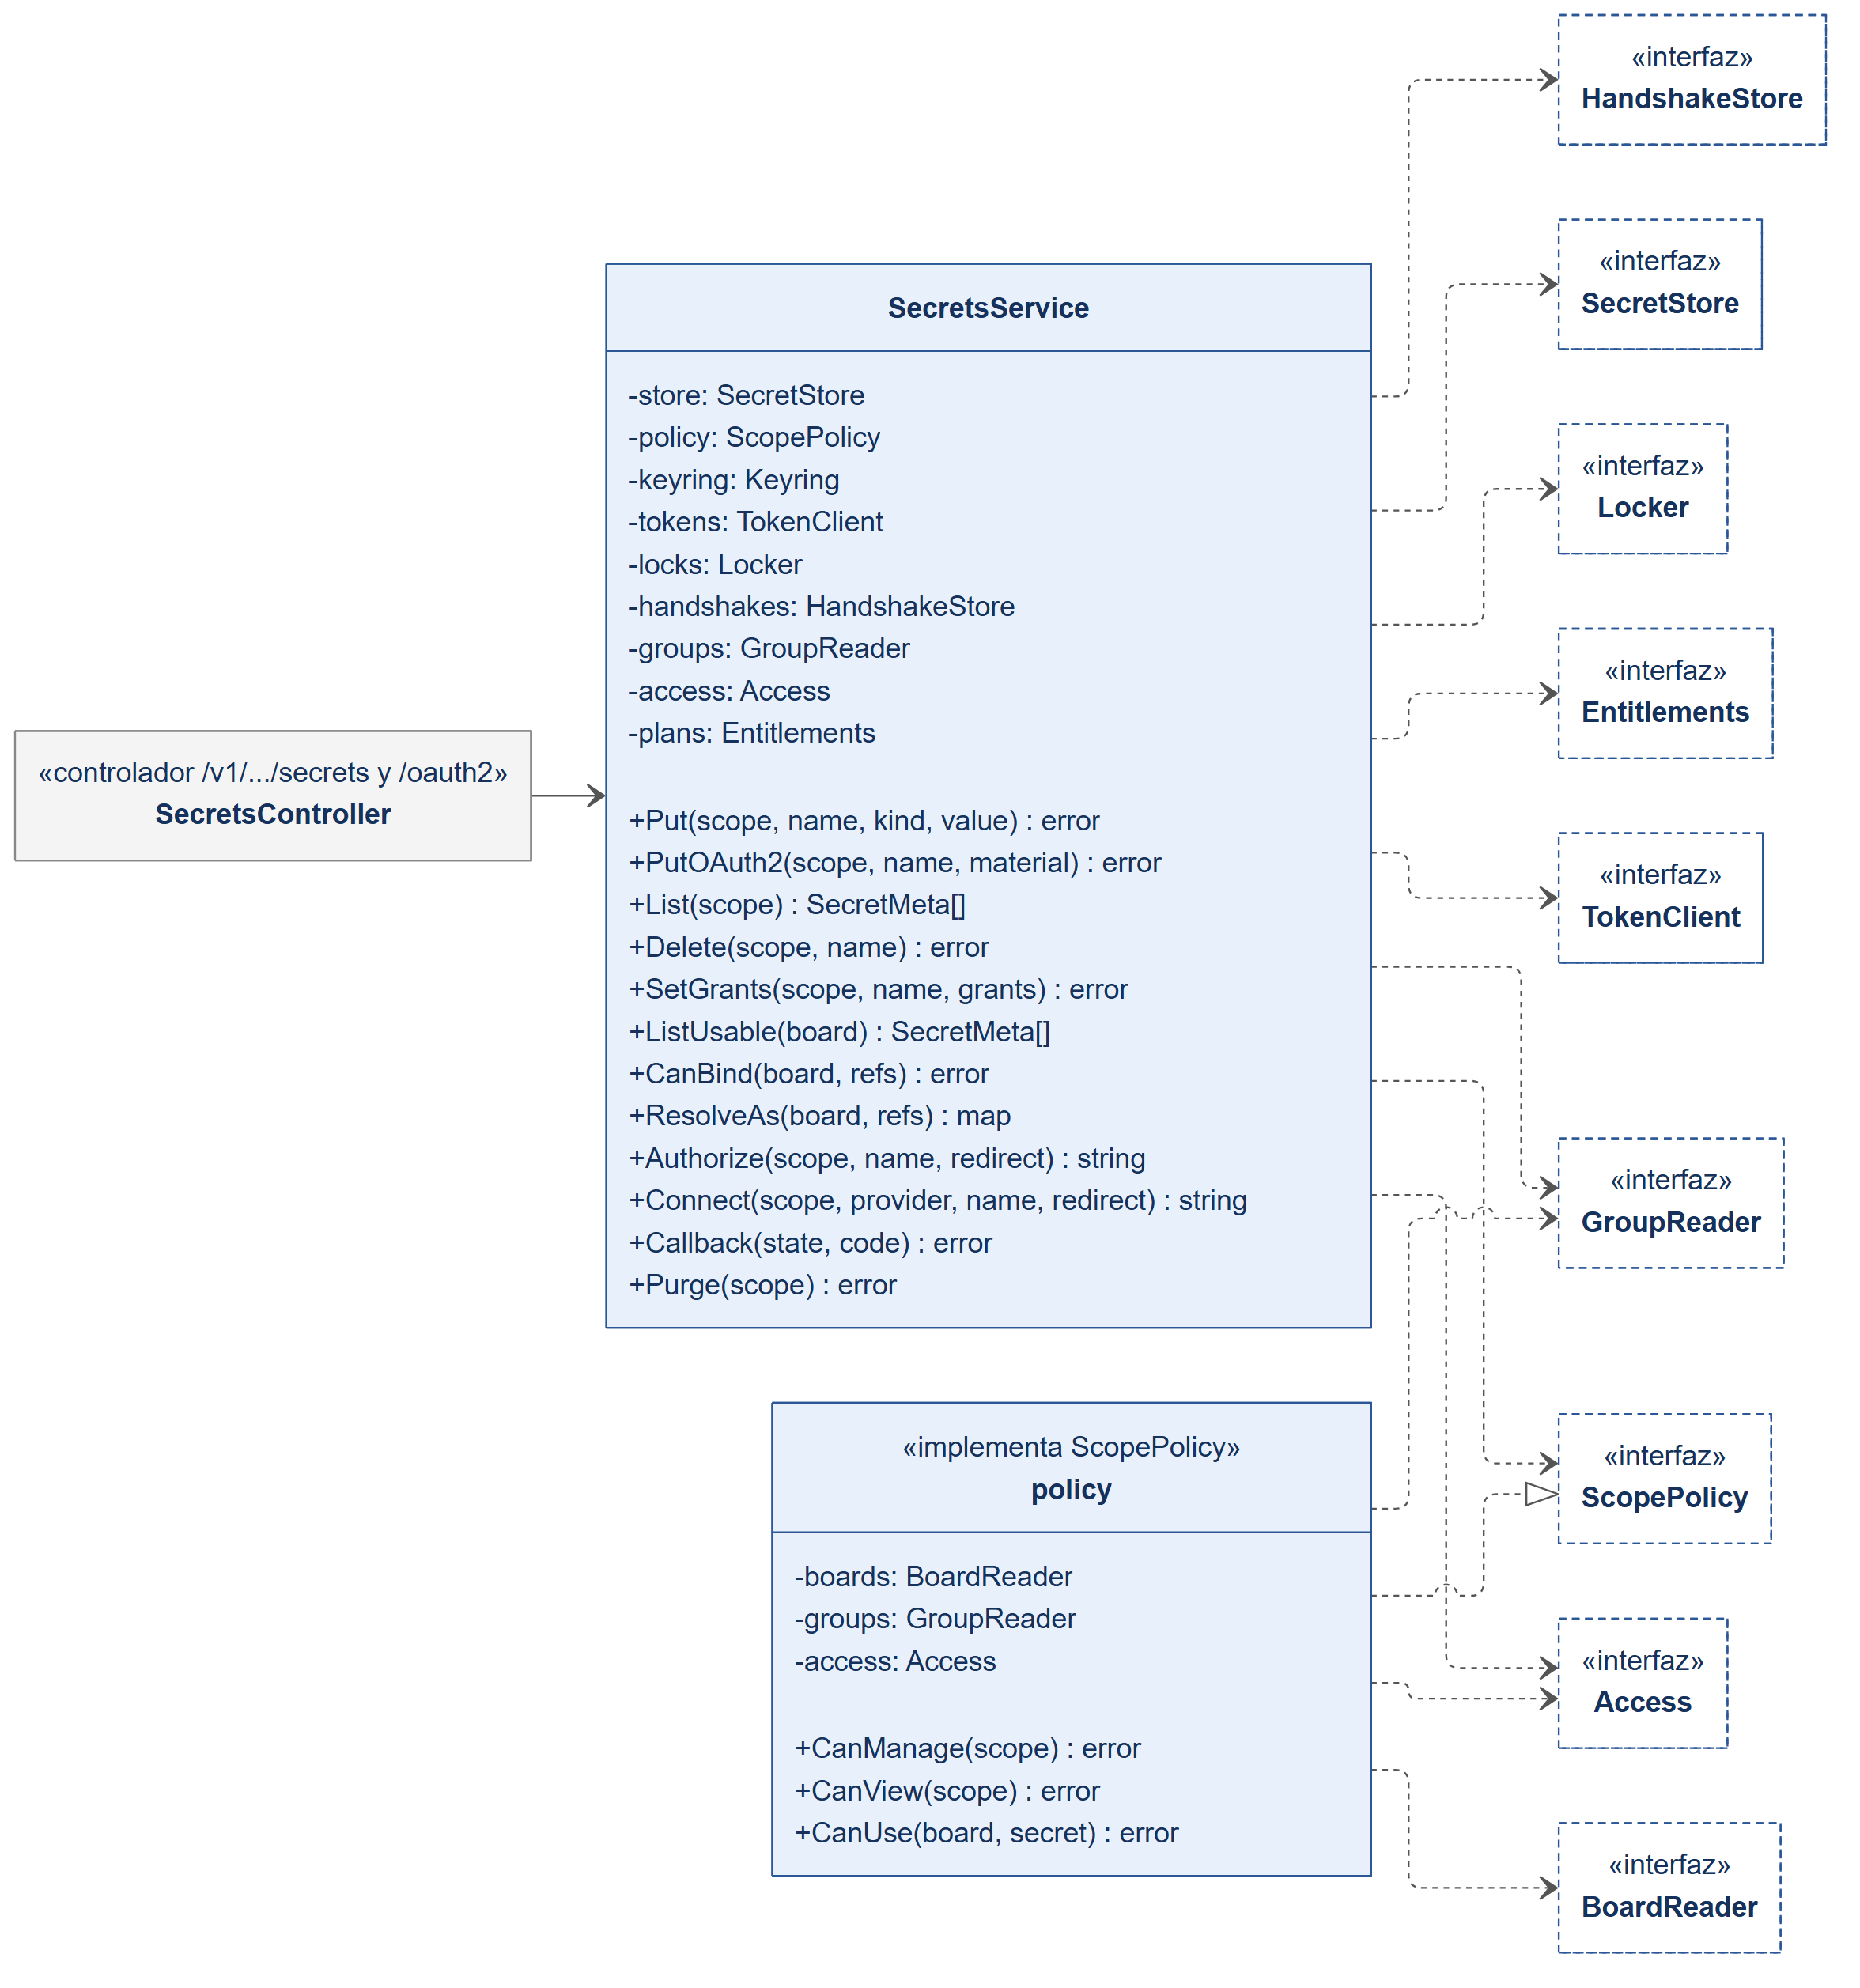
\includegraphics[width=0.92\textwidth]{figuras/fig24.png}
  \caption{Diagrama de clases de la bóveda de secretos}
  \label{fig:clases_boveda}
\end{figure}

\begin{tablaendpoints}{Endpoints de Secrets. \texttt{\{scope\}} corresponde a \texttt{/boards/\{id\}}, \texttt{/boards/\{id\}/members/\{user\}}, \texttt{/users/\{id\}} o \texttt{/groups/\{id\}}.}{tab:endpoints_secrets}
  GET & /\{scope\}/secrets & Listar la metadata de los secretos del ámbito. \\
  PUT & /\{scope\}/secrets & Crear o reemplazar un secreto (api\_key, bearer o basic). \\
  DELETE & /\{scope\}/secrets/\{name\} & Eliminar un secreto. \\
  PUT & /\{scope\}/secrets/\{name\}/grants & Definir con quién se comparte el secreto. \\
  PUT & /\{scope\}/oauth2 & Configurar una credencial OAuth2 con un cliente propio. \\
  GET & /\{scope\}/oauth2/authorize & Obtener la URL de consentimiento OAuth2. \\
  POST & /\{scope\}/oauth2/connect & Conectar una cuenta a través de un proveedor de la plataforma. \\
  GET & /boards/\{id\}/secrets/usable & Listar los secretos que el llamante puede vincular en el tablero. \\
  GET & /oauth2/providers & Listar los proveedores de la plataforma y si están configurados. \\
  GET & /oauth2/callback & Completar el consentimiento OAuth2 (solo quien lo inició). \\
  GET/PUT & /system/secrets & Listar o crear un secreto de sistema (solo administradores). \\
  DELETE & /system/secrets/\{name\} & Eliminar un secreto de sistema (solo administradores). \\
  PUT & /system/oauth2 & Configurar una credencial OAuth2 del ámbito sistema (solo administradores). \\
  PUT & /system/oauth2/clients & Configurar el cliente OAuth2 de un proveedor de la plataforma. \\
  GET & /system/keys & Listar el estado de las claves de datos. \\
\end{tablaendpoints}

Las credenciales OAuth2 pueden obtenerse con un cliente propio del usuario o a través de un proveedor administrado por la plataforma (Google, Discord), en cuyo caso el client id y el client secret se almacenan como secreto de sistema y se incorporan a la credencial únicamente en memoria. Los access tokens se renuevan automáticamente un minuto antes de su vencimiento, utilizando un lock distribuido en Redis para que dos ejecuciones concurrentes no consuman el mismo refresh token. Ningún handler devuelve jamás el valor de un secreto, un client secret ni un token. Cada secreto se descuenta del plan del usuario que paga su ámbito, registrado en \texttt{billed\_to}.

\section{Planes y facturación}
Este componente, materializado en los paquetes \texttt{entitlements} y \texttt{billing} y en el adaptador \texttt{mercadopago}, define qué permite cada plan y cobra las suscripciones de los planes pagos.

Cada usuario tiene un plan (\texttt{free}, \texttt{pro} o \texttt{max}) y una fecha de vencimiento opcional. Los límites de cada plan forman una única tabla en el código, que el frontend recibe para mostrarlos: cantidad de organizaciones, tableros por espacio, asientos, tarjetas por tablero, plantillas por ámbito, secretos y grupos, el tiempo mínimo de un resultado en caché, y si el plan permite forzar actualizaciones y usar tokens personales.

El servicio \texttt{entitlements} resuelve, para cada recurso, quién lo paga: un tablero personal lo paga su dueño, uno de organización el pagador de la organización, y un secreto el usuario indicado en \texttt{billed\_to}. Los demás servicios consultan este puerto antes de crear algo y, si el plan del pagador no lo admite, responden 402 con el nombre del límite alcanzado, su máximo y el plan vigente. Solo se rechazan las creaciones nuevas, de modo que una cuenta que baja de plan conserva lo que ya tiene.

El cobro se realiza mediante suscripciones mensuales de Mercado Pago, con un precio en pesos calculado a partir del precio en dólares de cada plan. Al suscribirse, el backend crea la suscripción y devuelve la URL del checkout del proveedor, que al finalizar redirige al frontend para sincronizarla. Cada cambio posterior llega por un webhook cuya firma HMAC se verifica, y el backend nunca confía en su contenido: ante cada notificación vuelve a leer la suscripción desde Mercado Pago. El plan queda vigente hasta cinco días después del próximo pago esperado, por lo que una suscripción cancelada o impaga vuelve sola al plan gratuito. Subir de plan se aplica de inmediato, mientras que bajarlo se aplica con la siguiente factura pagada.

Las clases que intervienen se muestran en la Figura~\ref{fig:clases_billing}. \texttt{EntitlementsService} implementa el puerto \texttt{Entitlements} que consultan los demás servicios, y para ello lee usuarios, organizaciones, tableros y grupos, y obtiene del puerto \texttt{Counter} los conteos de cada límite. \texttt{BillingService} depende del puerto \texttt{PaymentGateway}, implementado por el adaptador \texttt{Gateway} sobre el SDK de Mercado Pago, y de \texttt{SubscriptionStore} para guardar el estado conocido de cada suscripción.

\begin{figure}[H]
  \centering
  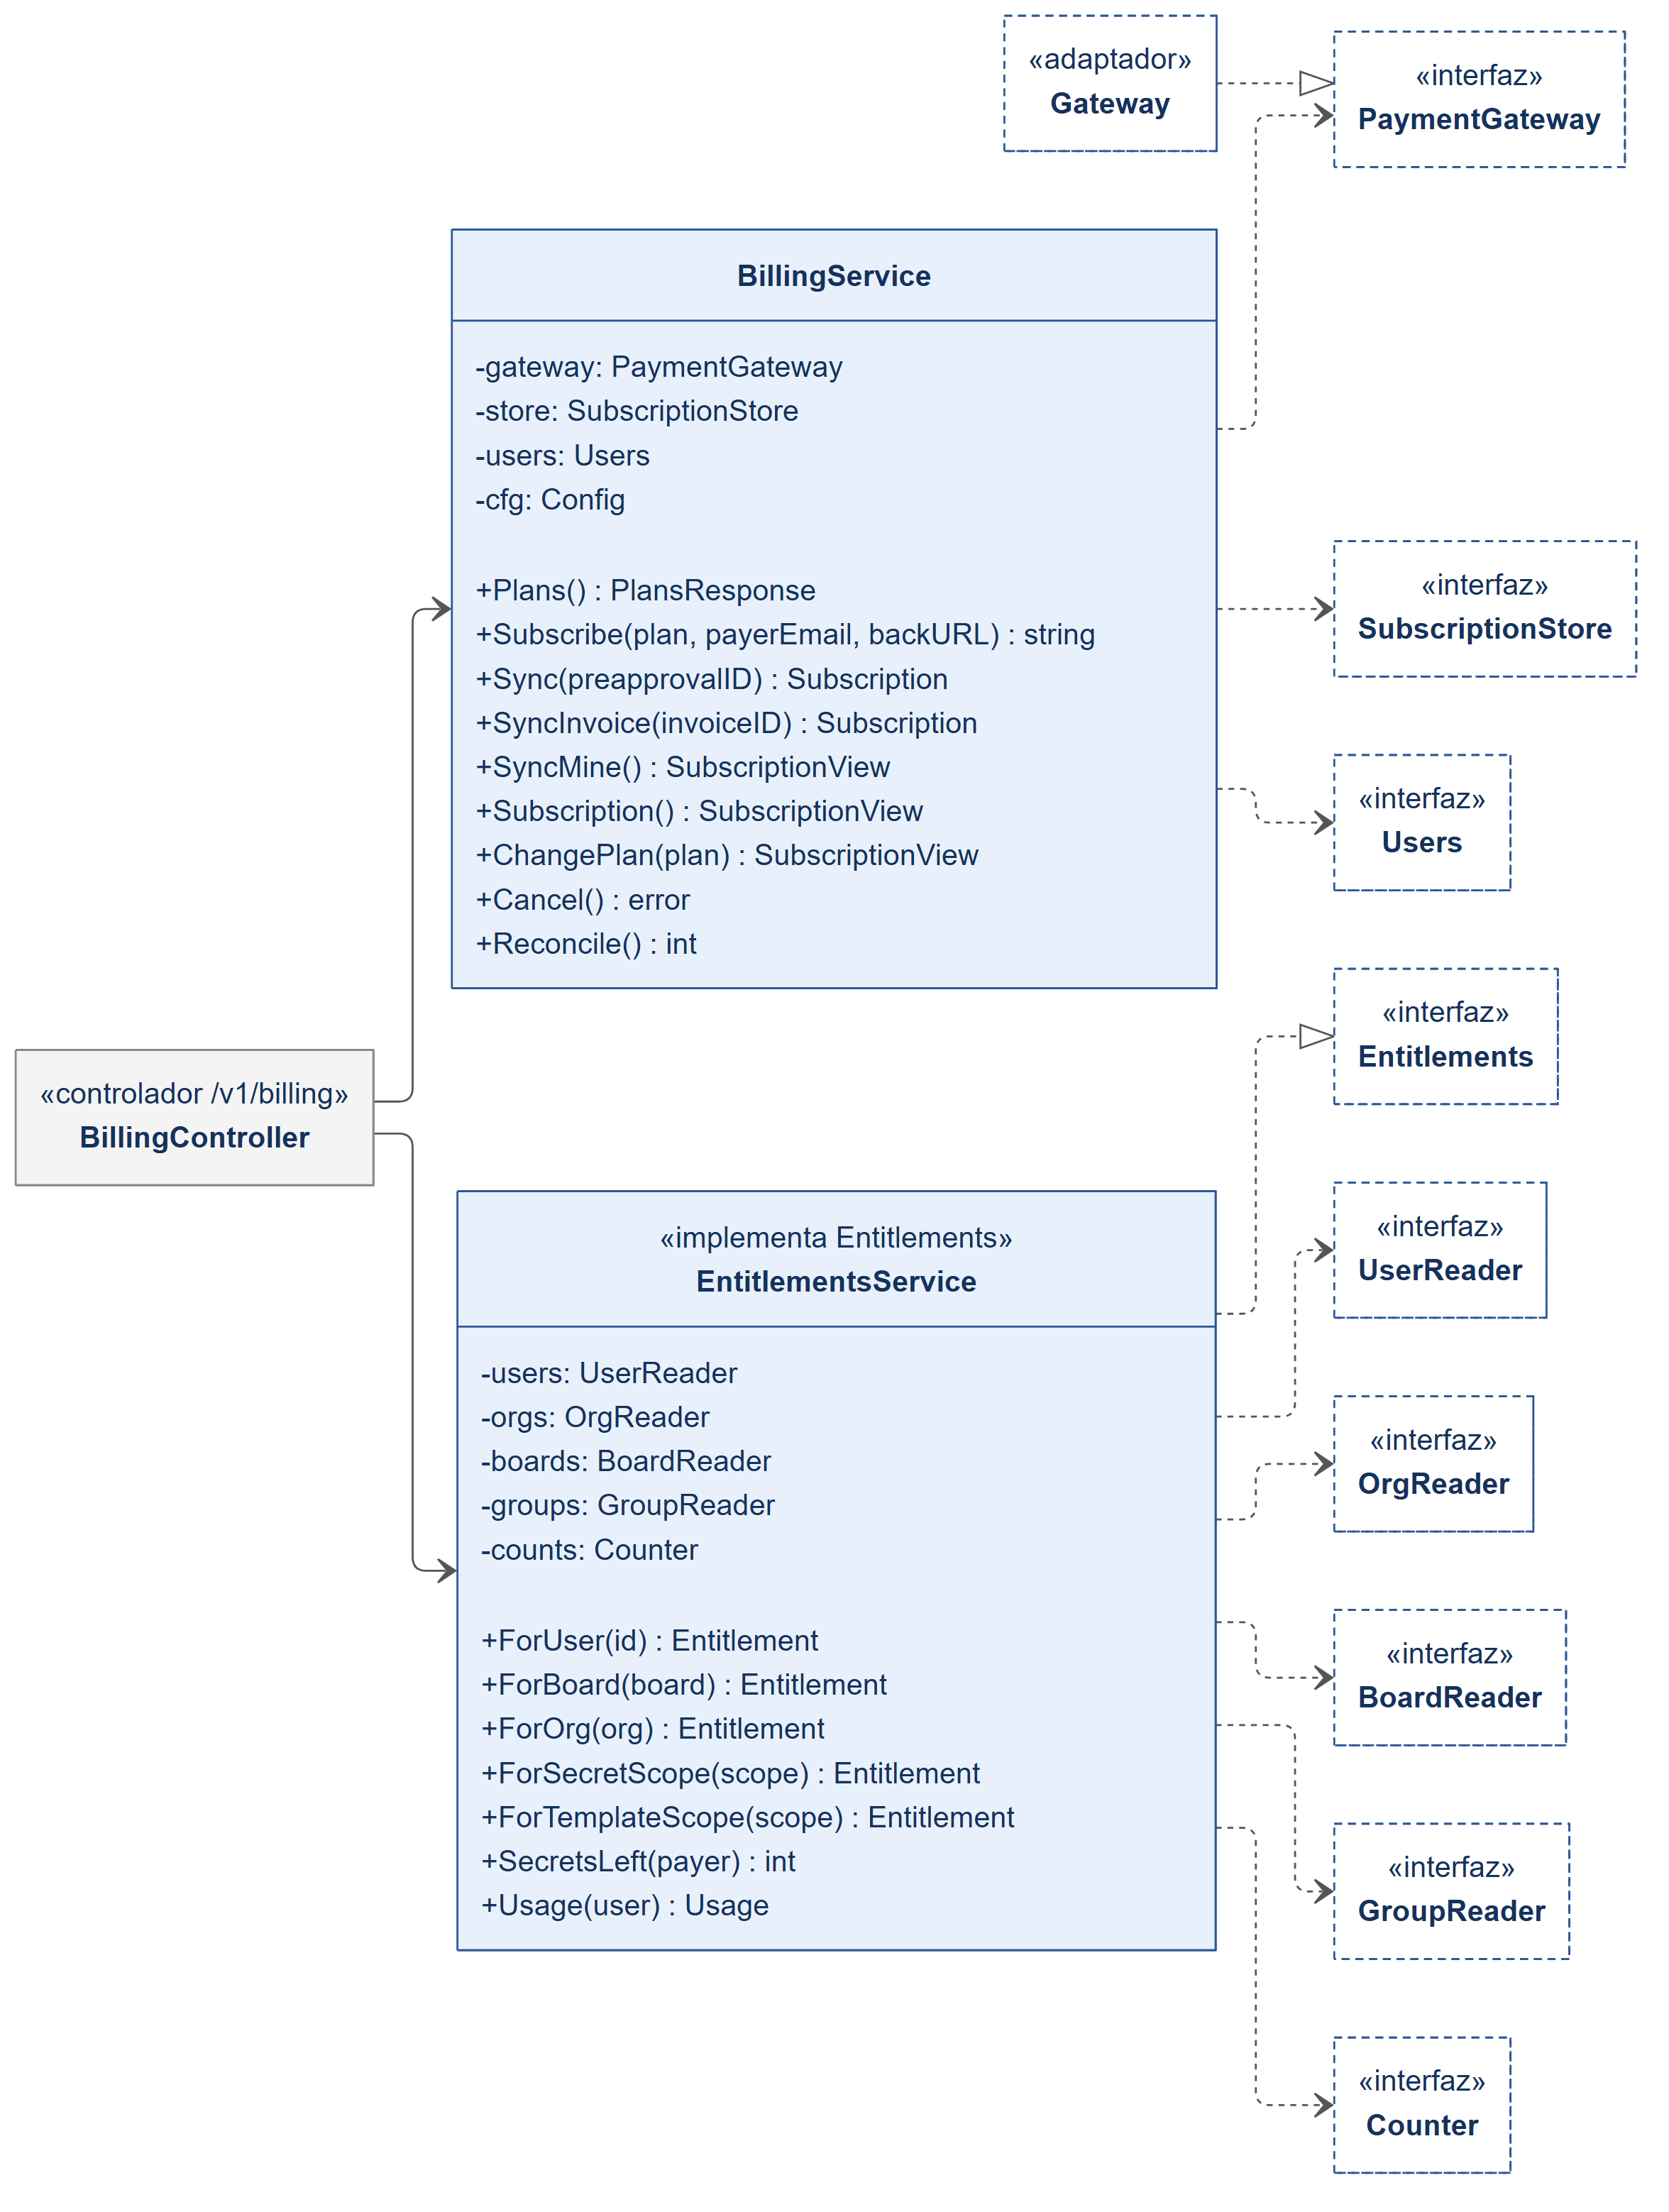
\includegraphics[width=0.85\textwidth]{figuras/fig41.png}
  \caption{Diagrama de clases de planes y facturación}
  \label{fig:clases_billing}
\end{figure}

Los endpoints de este componente se resumen en la Tabla~\ref{tab:endpoints_billing}.

\begin{tablaendpoints}{Endpoints de Billing}{tab:endpoints_billing}
  GET & /billing/plans & Listar los planes con sus límites y precios (público). \\
  POST & /billing/webhook & Recibir las notificaciones de Mercado Pago (público, con firma). \\
  GET & /billing/usage & Obtener el uso de la cuenta (organizaciones, grupos, secretos y plantillas). \\
  GET & /billing/subscription & Obtener el plan vigente y el estado de la suscripción. \\
  POST & /billing/subscribe & Iniciar una suscripción y obtener la URL del checkout. \\
  POST & /billing/sync & Sincronizar la suscripción tras volver del checkout. \\
  PUT & /billing/subscription & Cambiar de plan. \\
  DELETE & /billing/subscription & Cancelar la suscripción. \\
\end{tablaendpoints}

\section{Persistencia y caché}
Los adaptadores de persistencia y caché, en los paquetes \texttt{mongo} y \texttt{redis}, proveen las implementaciones concretas de los puertos de infraestructura de los que dependen los servicios.

El adaptador \texttt{mongo} implementa los puertos \texttt{Database}, \texttt{UserStore}, \texttt{GroupStore}, \texttt{OrgStore}, \texttt{SecretStore}, \texttt{KeyStore}, \texttt{AccessTokenStore}, \texttt{WellKnownStore}, \texttt{PostitTemplateStore} y \texttt{SubscriptionStore}, junto con las interfaces de solo lectura \texttt{UserReader}, \texttt{OrgReader}, \texttt{GroupReader} y \texttt{BoardReader}, encapsulando la lógica de persistencia descrita en los componentes anteriores, así como los conteos que necesita el servicio de planes para verificar cada límite. Al iniciar, \texttt{EnsureIndexes} crea de forma idempotente los índices de los que dependen las invariantes de unicidad, como el correo de cada usuario, el par \texttt{(scope, name)} de cada secreto o la existencia de una única clave de datos activa por ámbito.

Antes de crear los índices se ejecutan las migraciones, como el renombre de colecciones heredadas, y luego se carga el catálogo inicial de integraciones. En Vercel este paso no se ejecuta en cada arranque en frío, sino una única vez por despliegue de producción, mediante el comando \texttt{-migrate} durante la compilación.

El adaptador \texttt{redis}, por su parte, implementa el puerto \texttt{Caché} mediante las operaciones \texttt{FindPostItResult}, \texttt{AddPostItResult} y \texttt{DropPostItResult}, almacenando el último resultado de cada tarjeta bajo su identificador, con un tiempo de vida igual a su rate, y descartándolo cuando la tarjeta se edita o se elimina. Además, implementa las sesiones de refresco (claves \texttt{session:}, \texttt{spent:}, \texttt{family:} y \texttt{user-families:}), los límites de tasa (\texttt{rate:}, por ejemplo para inicios de sesión, invitaciones, creación de tokens y actualizaciones forzadas), los locks distribuidos (\texttt{lock:}) y los handshakes de los flujos OAuth2 (\texttt{oauth-handshake:}). La presencia de los usuarios en cada tablero (\texttt{board:\{id\}:online}) la escribe únicamente el servicio de tiempo real.

La relación entre estos adaptadores y los puertos que satisfacen se ilustra en la Figura~\ref{fig:adaptadores_persistencia}. Gracias a esta inversión de dependencias, cualquiera de estas tecnologías podría reemplazarse sin alterar la lógica de negocio. Cada círculo representa una interfaz provista por el adaptador, según la notación de UML.

\begin{figure}[H]
  \centering
  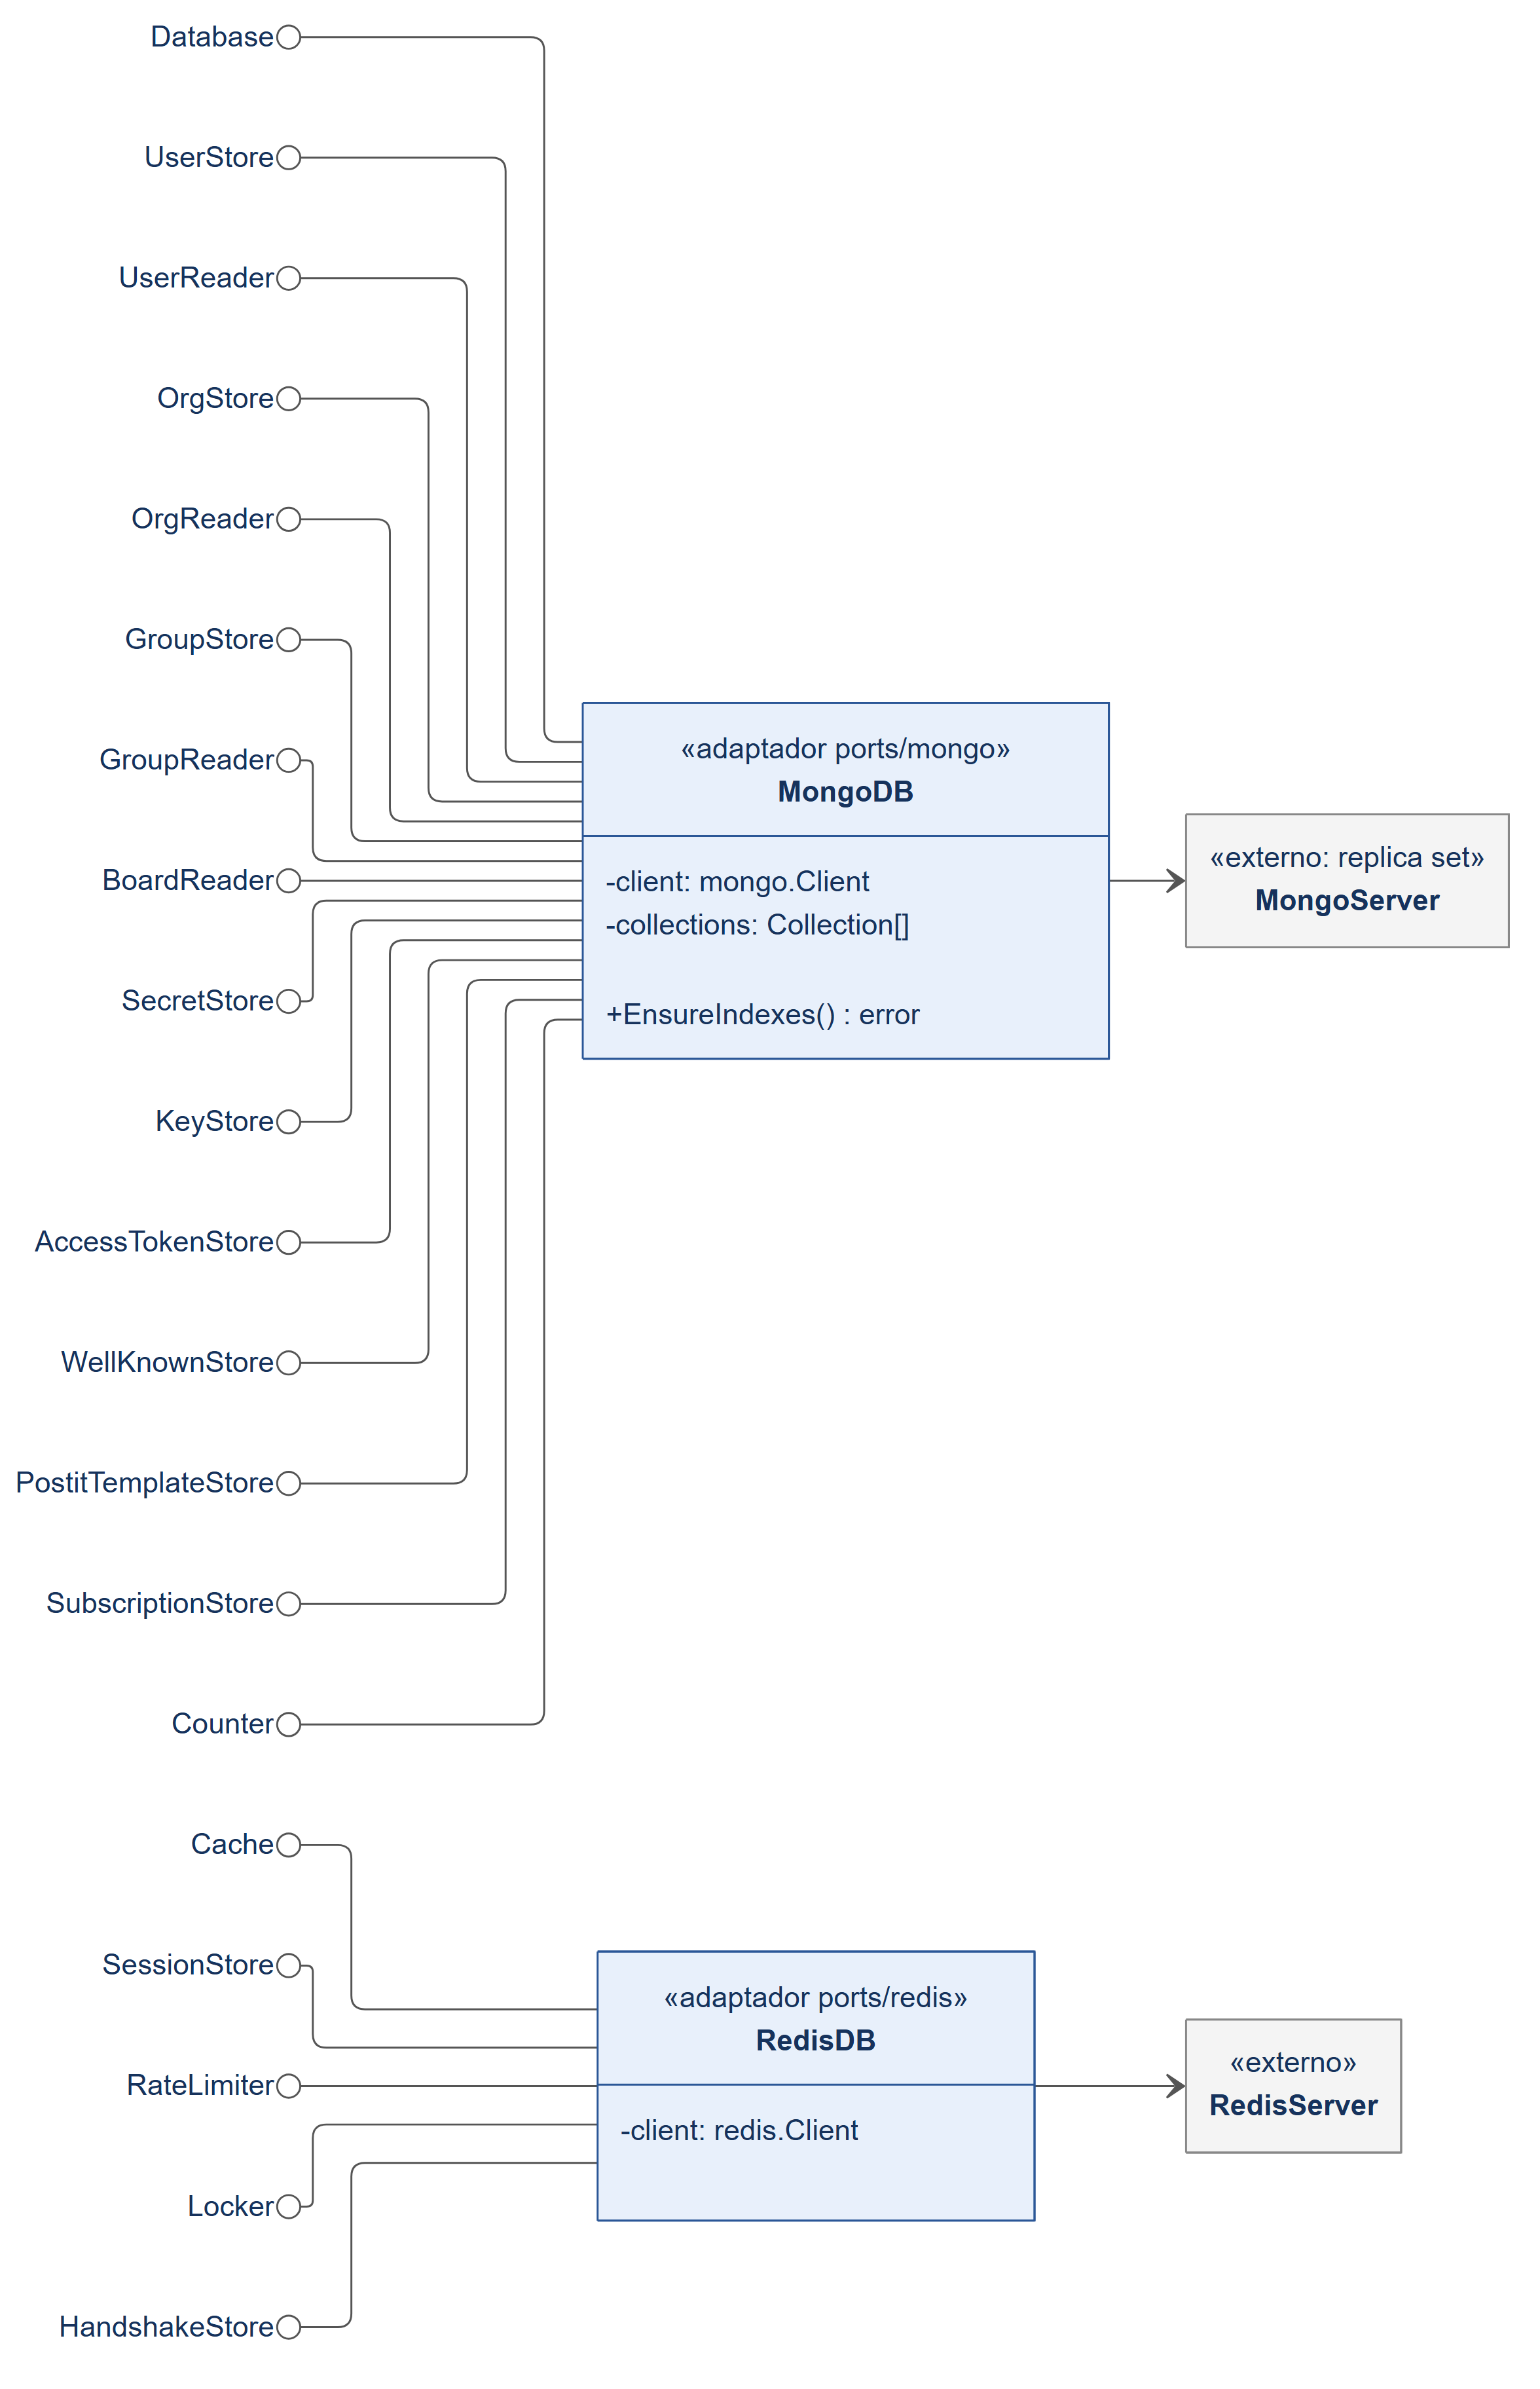
\includegraphics[width=0.78\textwidth]{figuras/fig25.png}
  \caption{Adaptadores de persistencia y puertos que implementan}
  \label{fig:adaptadores_persistencia}
\end{figure}

\section{Estrategia de actualización y caché}
A diferencia de los componentes anteriores, la actualización de las tarjetas no constituye un paquete independiente, sino una capacidad transversal que emerge de la colaboración entre el motor de tarjetas, el adaptador de caché y el frontend. Su objetivo es garantizar que las tarjetas reflejen el último dato disponible sin intervención del usuario, según lo establecido por el RF-09.

El mecanismo principal es un caché por tarjeta: al ejecutar una tarjeta, el servicio consulta primero Redis mediante \texttt{FindPostItResult} y, si existe un valor cacheado, lo devuelve sin tocar la fuente externa; en caso contrario, ejecuta el pipeline del executer y persiste el resultado con \texttt{AddPostItResult}, que aplica un \texttt{SET} con expiración igual al rate de la tarjeta o, si es menor, al tiempo mínimo que fija el plan, de modo que el tiempo de vida natural del dato coincide con su frecuencia de actualización sin que un rate muy bajo multiplique las consultas. Así, todos los usuarios que observan una misma tarjeta comparten un único resultado y la API externa se consulta como máximo una vez por período. Editar o eliminar la tarjeta descarta su resultado, y en el plan Max el usuario puede forzar una nueva ejecución. Este recorrido corresponde al diagrama de secuencia de la Figura~\ref{fig:seq_ejecucion}.

A esto se suma el header \texttt{Cache-Control: private, max-age=10} (o \texttt{no-store} en una actualización forzada) en la respuesta de ejecución, que permite que el navegador absorba parte de la carga, y el servicio de tiempo real, que notifica a cada cliente los cambios estructurales del tablero, como tarjetas agregadas, movidas o reconfiguradas, para que vuelva a cargarlo sin necesidad de polling.

\section{Notificaciones por correo}
El adaptador \texttt{mail} implementa el puerto \texttt{Mailer}, encargado de enviar los correos de verificación de cuenta y de recuperación de contraseña, así como el aviso que recibe el titular de una cuenta cuando alguien intenta registrarse con su correo, lo que evita revelar en la respuesta del registro si una dirección ya existe. Cada correo se renderiza a partir de plantillas embebidas en el binario, una por idioma, y se envía en el idioma preferido del destinatario. Al iniciar, el servicio verifica que cada plantilla exista en todos los idiomas soportados, rechazando el arranque en caso contrario.

El envío se delega en un \texttt{Sender} intercambiable: con la variable \texttt{RESEND\_API\_KEY} configurada se utiliza Resend, mientras que sin ella los correos se vuelcan al log, lo que permite desarrollar localmente sin un proveedor externo.

La Figura~\ref{fig:clases_mail} muestra las clases del adaptador. \texttt{Mailer} implementa el puerto del mismo nombre y combina las plantillas, que generan el asunto y los cuerpos en texto y HTML, con un \texttt{Sender}, cuya implementación se elige al iniciar según la configuración.

\begin{figure}[H]
  \centering
  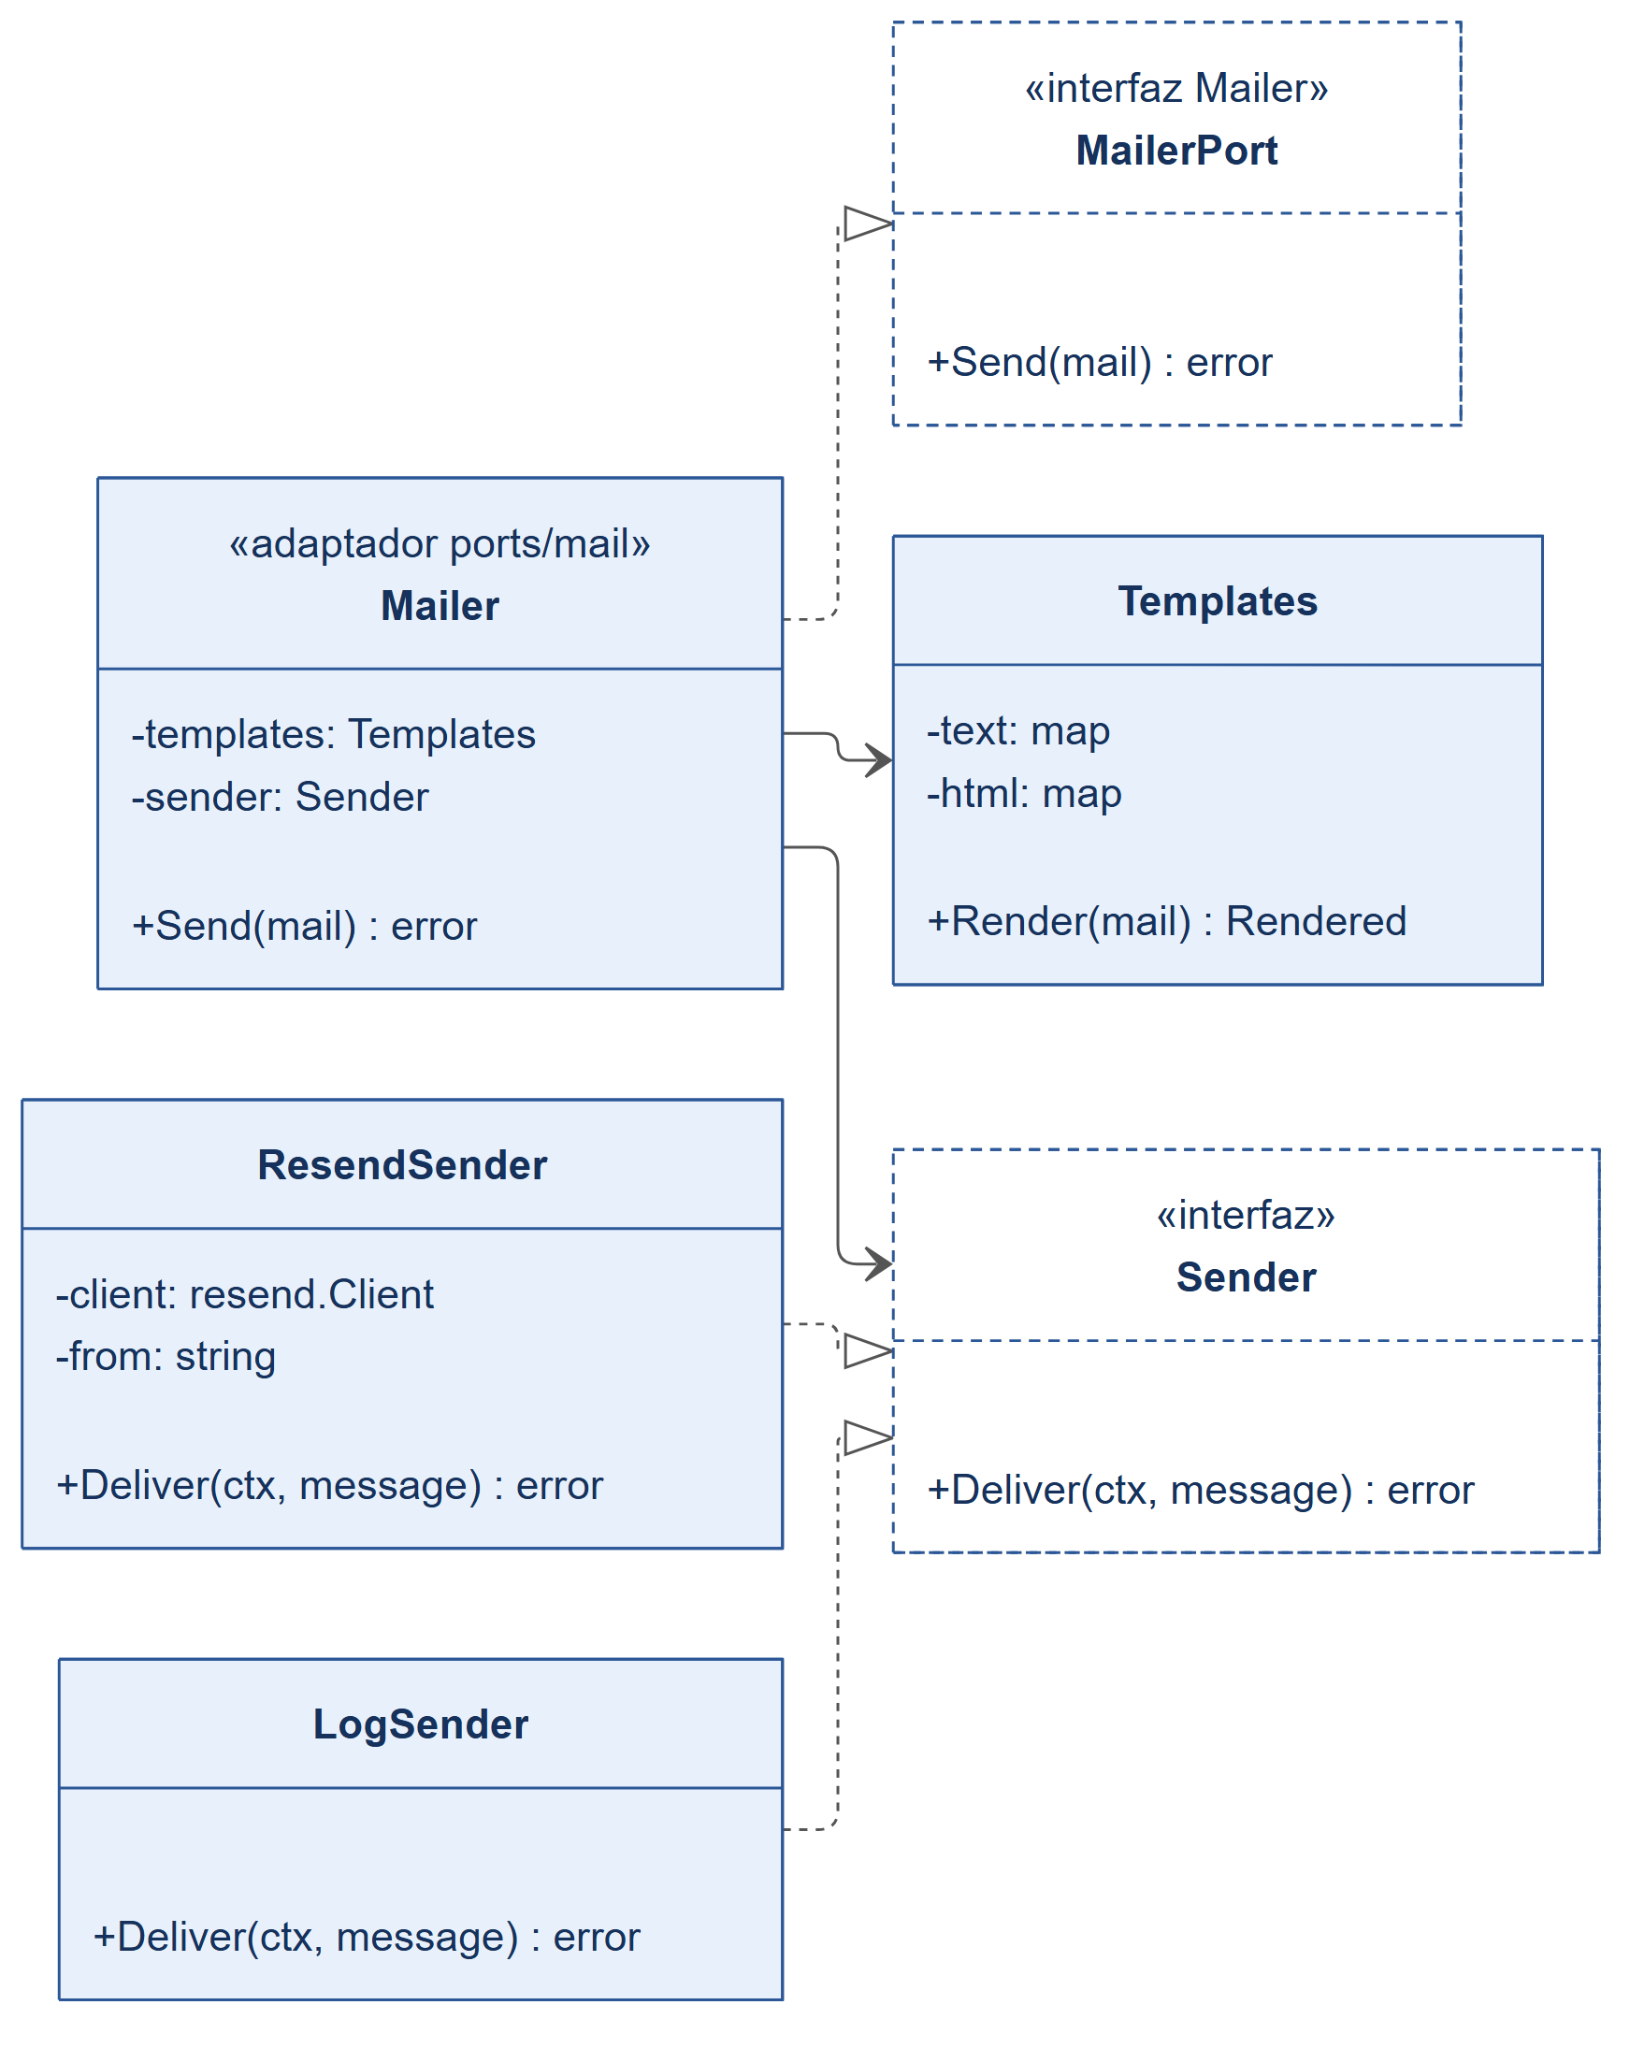
\includegraphics[width=0.72\textwidth]{figuras/fig26.png}
  \caption{Diagrama de clases del adaptador de correo}
  \label{fig:clases_mail}
\end{figure}

\section{Tiempo real}
El servicio de tiempo real, en la carpeta \texttt{realtime}, es un proceso Node independiente del backend encargado de propagar los cambios de un tablero a todos los usuarios conectados. Escucha la colección \texttt{boards} mediante un change stream de MongoDB y, ante cada actualización, emite un evento \texttt{update} a la sala de \texttt{socket.io} correspondiente al tablero.

Al conectarse, el cliente envía su token de acceso y el servicio consulta al backend \texttt{GET /boards/\{id\}} con ese mismo token: si no obtiene un 200 con un rol, rechaza la conexión. De esta forma, el servicio nunca verifica un JWT por sí mismo y el backend sigue siendo la única autoridad de autorización. Un minuto antes de que el token expire, el servidor solicita uno nuevo y vuelve a verificar el rol, de modo que un miembro removido pierde las actualizaciones a más tardar en la siguiente renovación. Si el cliente no presenta un token nuevo dentro de los treinta segundos posteriores al vencimiento, se lo desconecta.

La presencia de los usuarios en cada tablero se mantiene en el hash \texttt{board:\{id\}:online} de Redis, mientras que los cursores se comparten de manera peer-to-peer mediante WebRTC (PeerJS), sin pasar por el servidor. La entrada de presencia expira veinte minutos después de la última conexión o renovación.

La organización interna del servicio se representa en la Figura~\ref{fig:modulos_realtime}. El módulo \texttt{mongo} recibe los cambios del change stream y se los entrega a \texttt{socket}, que administra las salas. Este último consulta los roles a través de \texttt{auth}, que a su vez interroga al backend, y registra la presencia mediante el módulo \texttt{redis}.

\begin{figure}[H]
  \centering
  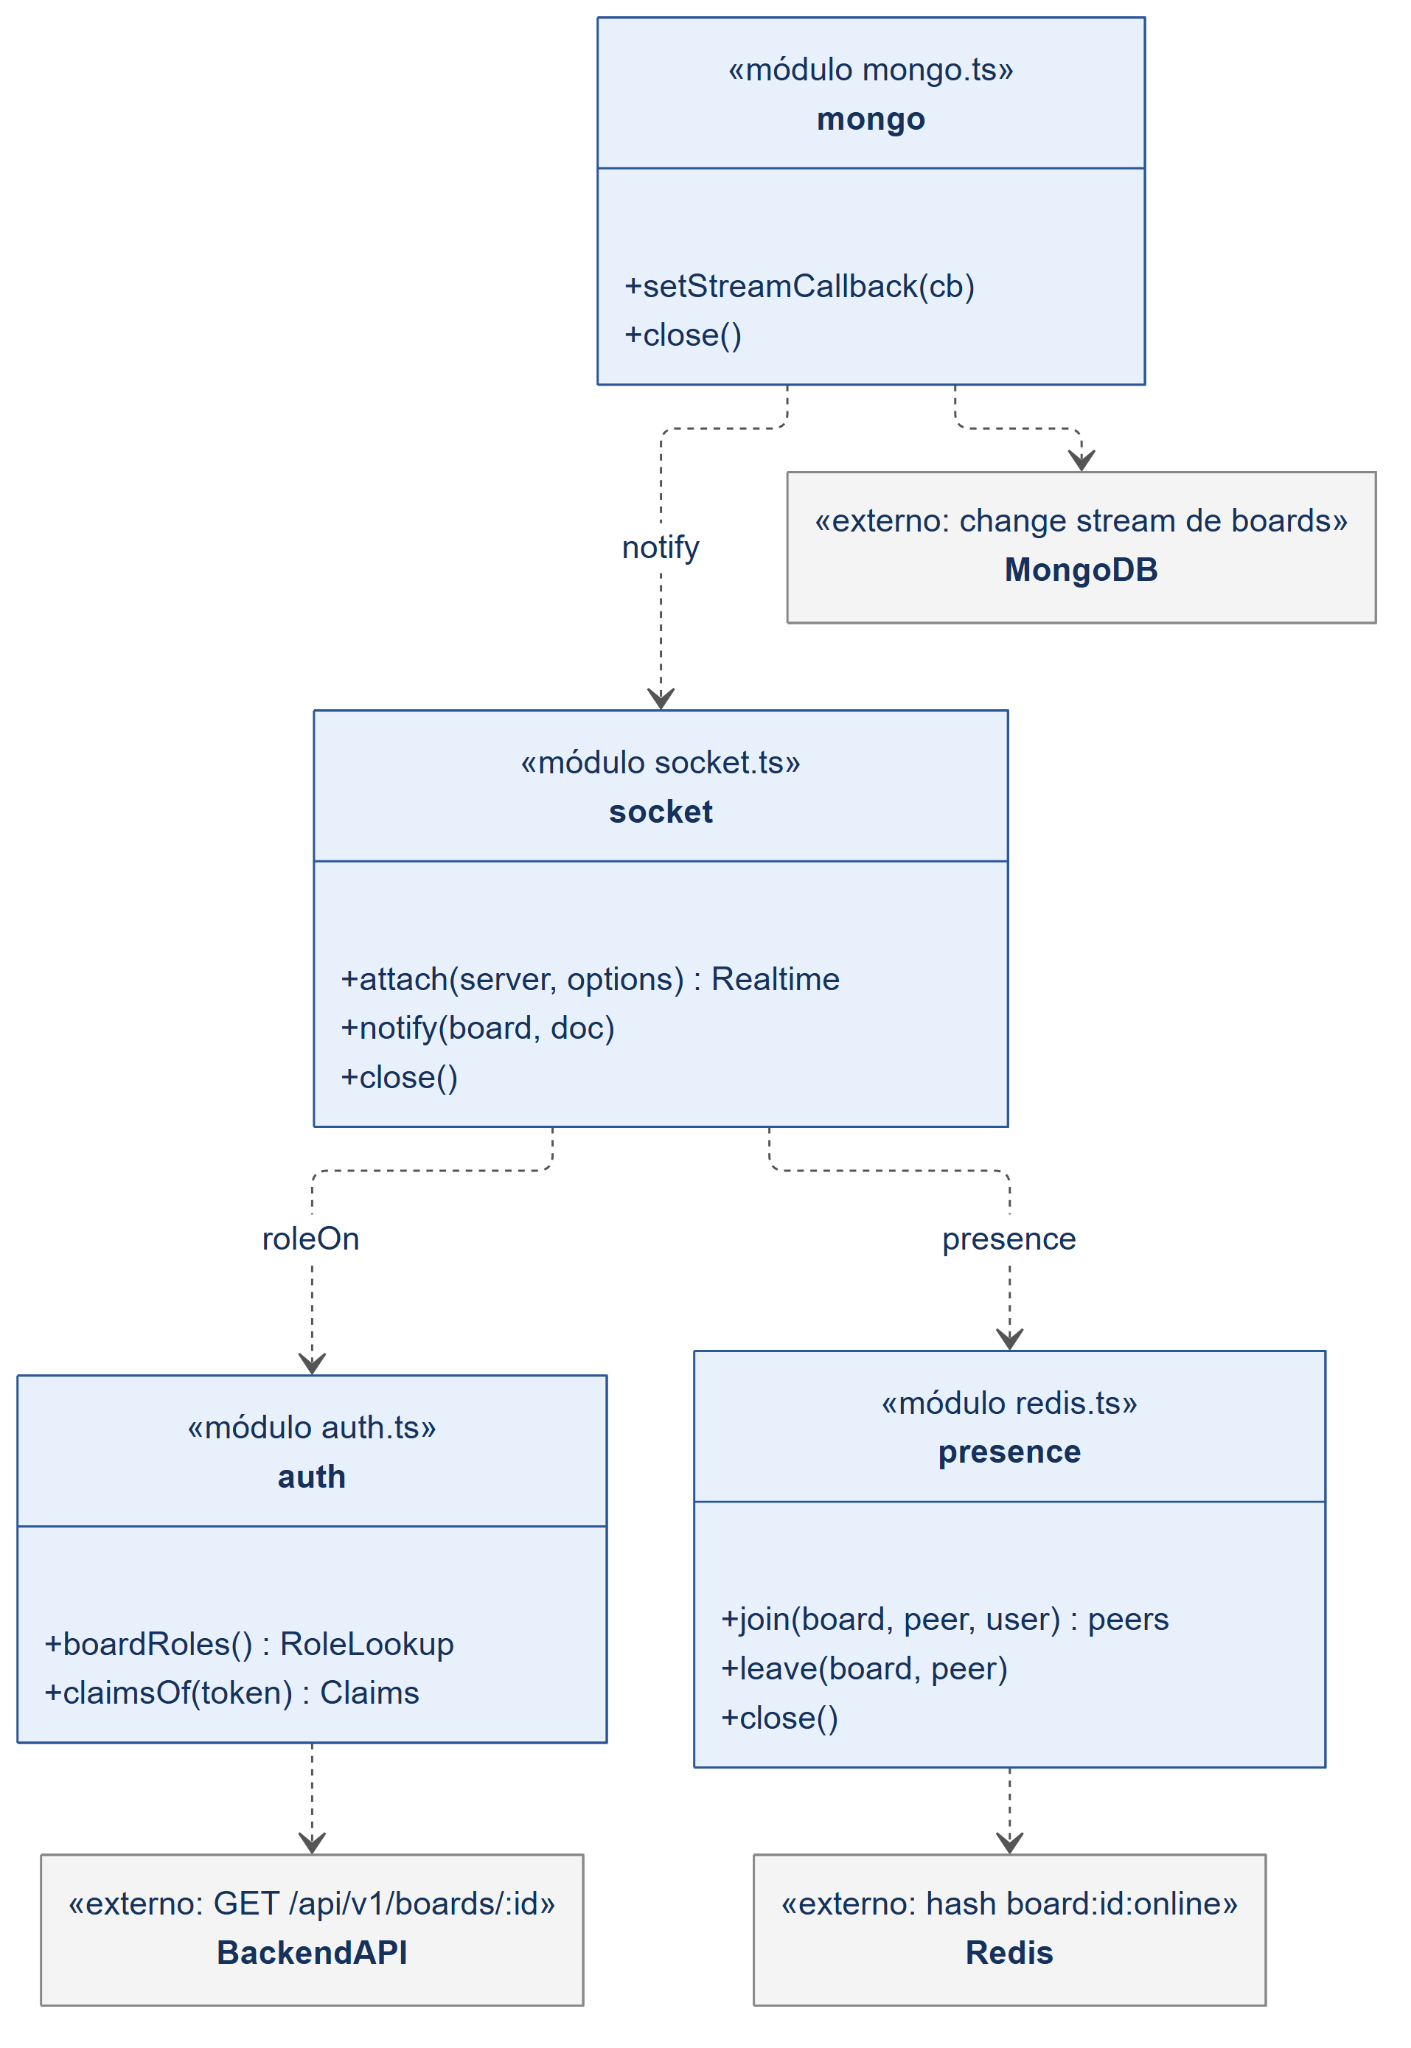
\includegraphics[width=0.75\textwidth]{figuras/fig27.png}
  \caption{Módulos del servicio de tiempo real}
  \label{fig:modulos_realtime}
\end{figure}